\chapter{The ND-LAr Cryostat}
\label{ch:cryostat}


%%%%%%%%%%%%%%%%%%%%%%%%%%%%%%%%
\section{Overview of the Cryostat}
\label{sec:cryost-ovvw}
This section covers the \dword{ndlar} cryostat. The cryostat is responsible for maintaining the \dword{lar} cryogenic environment required for the \dword{lartpc} modules that compose the \dword{ndlar}.  Similar to other large cryostats for \dwords{lartpc}, this cryostat uses a stainless steel membrane containment system, developed for the storage of liquified natural gas. The stainless steel membrane is corrugated to relieve strain resulting from temperature-related expansion and contraction. The insulation layer comprises multiple layers of polyurethane foam as well as a secondary steel barrier that can contain the liquid cryogen in the event of primary membrane failure. This inner structure is surrounded by a room-temperature (warm) structure that consists of a continuous 10\,mm thick steel vapor barrier backed by a structural frame of steel columns and beams. On one side of the cryostat, a composite window replaces the steel structure in order to limit the impact on crossing muons. The external superstructure supports the hydrostatic and pressure loads of the \dword{lar}. 

Uniquely, relative to most membrane cryostats for \dword{lar}, it is mounted to the \dword{duneprism} movement system, which will translate the cryostat along the length of the Near Site cavern hall.  Another unique feature is a low-density window construction on the downstream cryostat wall, designed to minimize attenuation of muons that exit the active region of the \dword{lartpc} array. The \dword{lar} cryostat is shown in the Near Site cavern in Figure~\ref{fig:cavern-cryostat}

\begin{dunefigure}[LAr cryostat in Near Site cavern layout]{fig:cavern-cryostat}
{LAr cryostat in Near Site cavern layout.}
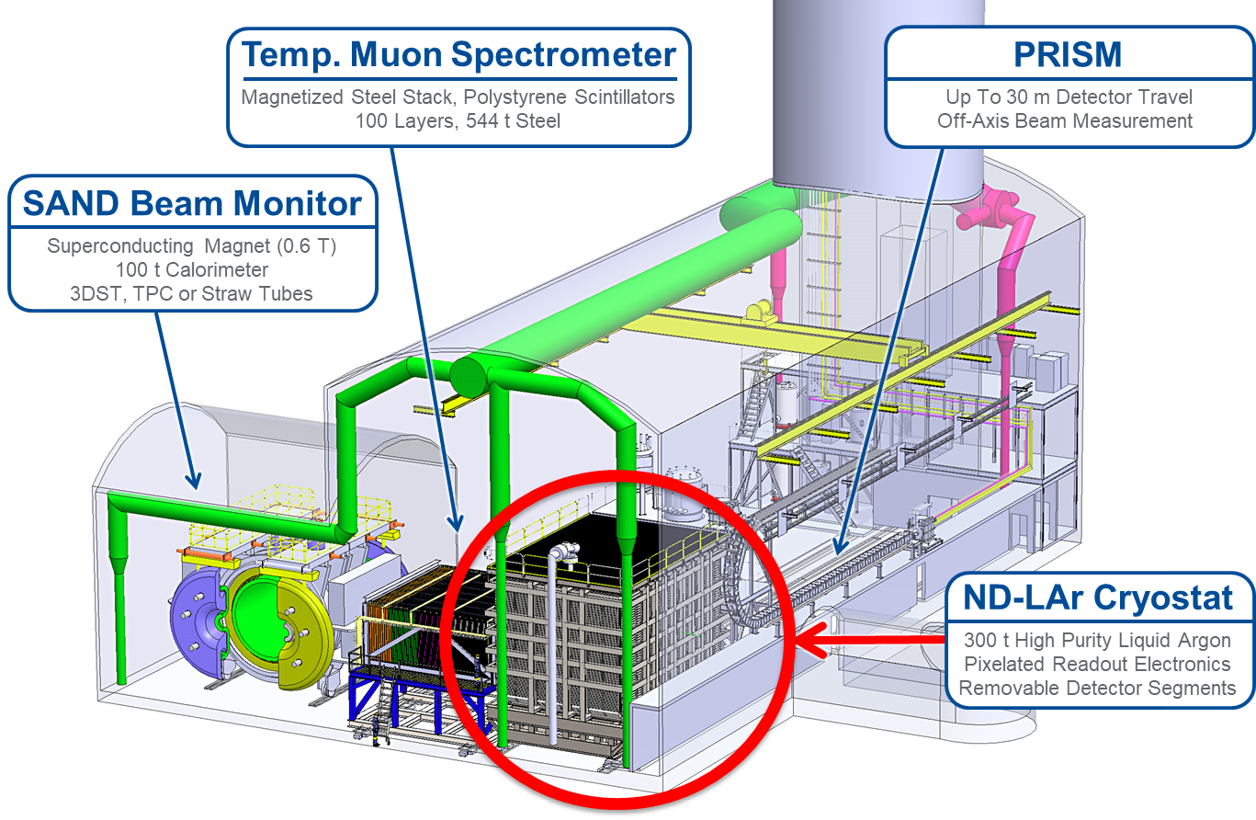
\includegraphics[width=0.95\textwidth]{graphics/cryostat/cavern-cryostat.png}
\end{dunefigure}

The following sections cover the design and requirements of the cold and warm containment structures, roof sections, interfaces, risks, schedule and installation activities.

%%%%%%%%%%%%%%%%%%%%%%%%%%%%%%%%%%%%
\section{Principle of Operation}
\label{sec:cryost-ovvw-prinoper}

The \dword{ndlar} cryostat provides the required operating environment for the \dword{lartpc} array.  The top lid hosts virtually all services to and from the inner cryogenic environment, as well as many of the exterior electronics that operate at ambient temperature.  The \dword{ndlar} cryostat is a super-structure consisting of a steel beam exterior and stainless steel containment membrane interior; with an insulation layer sandwiched between the two.  

%%%%%%%%%%%%%%%%%%%%%%%%%%%%%%%%%%%%
\section{Design Requirements and Parameters}
\label{sec:cryost-ovvw-reqparam}

\subsection{Requirements}
\label{sec:cryost-ovvw-req}

The \dword{ndlar} cryostat is designed to satisfy the requirements imposed on it by the \dword{ndlar} and the overall physics program; these are shown in Table~\ref{tab:table-cryost-reqs}.

\fixme{The label is intended for cross-referencing; probably not useful in the table itself. It's needed in the Excel file to generate the latex, if we go that route. We can discuss. Anne}
\begin{dunetable}
[Cryostat Requirements]
{p{.13\textwidth}p{0.22\textwidth}p{.18\textwidth}p{.25\textwidth}p{.10\textwidth}}
%{lllll}
{tab:table-cryost-reqs}
{LAr Cryostat Requirements}
Label & Description & Specification & Rationale & Validation \\ \toprowrule
cryostat-inner-dimen & The ND LArTPC cryostat shall be large enough to host the LArTPC array & $> (3 \times 5 \times 7)\mbox{m}^3$ & The ND LArTPC cryostat inner dimensions must be large enough to host the ND LArTPC detector system & Inspection \\ \colhline
downstream-pass-mat & Downstream wall average mass shall be minimized to mitigate attentuation exiting neutrino-induced muons & $< 50 g/\mbox{cm}^2$ & The downstream material of the ND LArTPC cryostat (cold structure, warm structure, plus inactive argon when filled) must not substantially attentuate neutrino-induced muons exiting the ND LArTPC & Simulation \\ \colhline
cryostat-robust-prism & Shall be sufficiently robust such that off-axis (PRISM) movements do not substantially impact cryostat performance & ?? & The ND LArTPC Cryostat shall be sufficiently robust such that off-axis (PRISM) movements do not substantially impact cryostat performance & Simulation, Analysis \\ 
\end{dunetable}

\subsection{Parameters}
\label{sec:cryost-ovvw-param-dim}

The important design parameters are given in Table~\ref{tab:table-cryost-params}. 

\fixme{parameters table by hand or generated?}

%\begin{itemize}
%\item Size requirements
%\item Containment requirements
%\item Capabilities
%\item Operating parameters  
%\end{itemize}

\begin{dunetable}
[Cryostat Parameters]
{p{.25\textwidth}p{0.25\textwidth}p{.50\textwidth}}
%{lll}
{tab:table-cryost-params}
{LAr Cryostat Design Parameters}
Design Parameter            & Value & Notes \\ \toprowrule
Inner Volume                & $5500\times 6000 \times 9000 \mbox{mm}^2$ & height $\times$ width $\times$ length \\ \colhline
Tank Capacity               & 340 metric tonnes & Defined by cold membrane vessel \\ \colhline
Residual Heat Input         & $<10$ $\mbox{W}/\mbox{m}^2$       & \\ \colhline
Insulation Density          & 90  $\mbox{kg}/\mbox{m}^3$& \\ \colhline
Insulation Thickness        & 800 $\mbox{mm}$           & Includes primary and secondary membrane; an insulation thickness of 600\,mm is desirable if RHI satisfied
\\ \colhline
Maximum Allowable Pressure  & 350 $\mbox{mbarg}$        & Set point of the cryostat pressure safety valve\\ \colhline
Cavern Ambient Pressure     & 1020.355 $\mbox{mbara}$   & Cryostat pressure safety valves shall be set at 350\,mbarg with respect to ambient pressure\\ \colhline
Operating Temperature     & 86K to 90K  & \\
\end{dunetable}

\fixme{define RHI}


%%%%%%%%%%%%%%%%%%%%%
%\subsection{Dimensions}
%\label{sec:cryost-ovvw-param-dim}

The overall cryostat dimensions are based on the required volume of \dword{lar} for the \dword{ndlar}, and the structure required to support it.  The nominal external and internal dimensions for the cryostat are shown in Figure~\ref{fig:cryo-dim} and listed in Table~\ref{tab:table-cryost-dimensions}.

\begin{dunefigure}[Cryostat dimensions]{fig:cryo-dim}
{Cryostat internal and external dimensions in mm. Section A-A shows all widths and warm structure heights, B-B shows all  lengths and the inner membrane height. The hatched region is the insulation layer (1600\,mm thick on the sides and 1800\,mm thick on the bottom).}
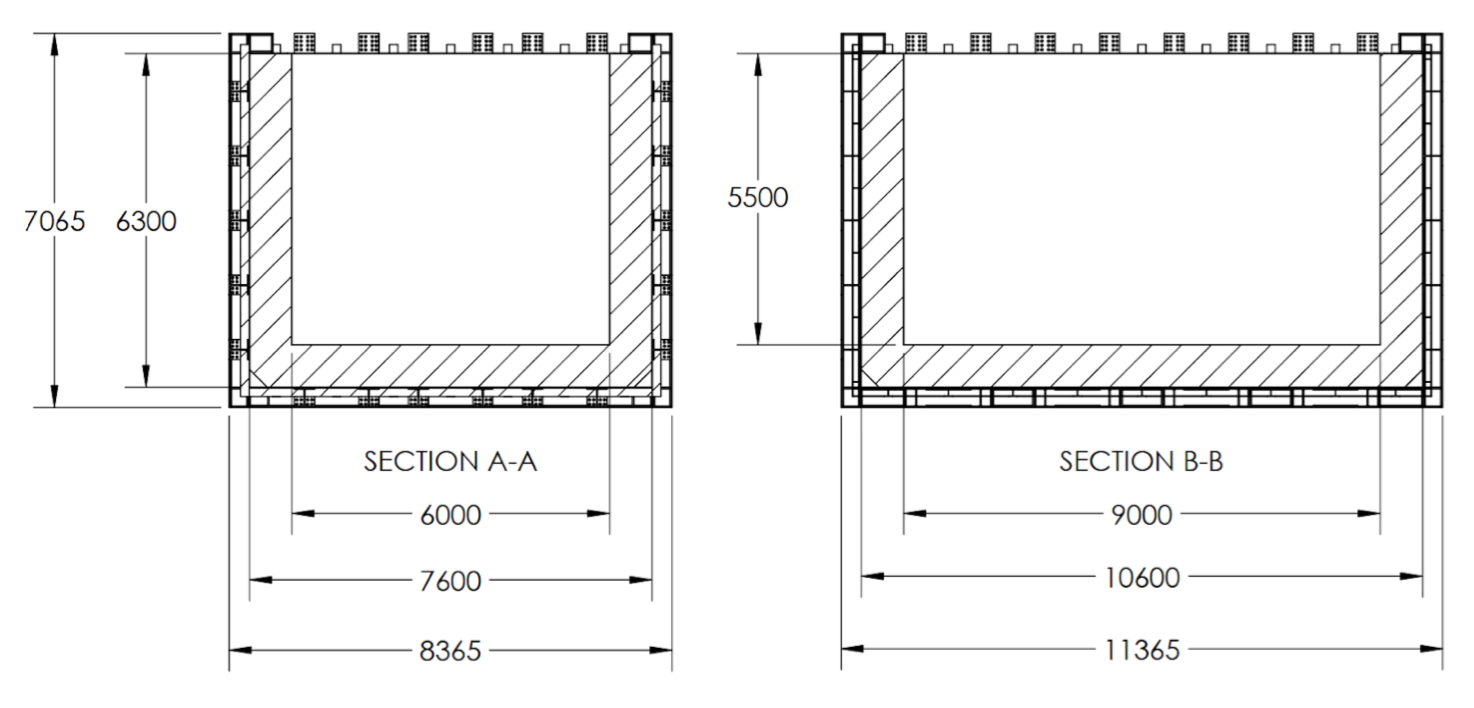
\includegraphics[width=0.95\textwidth]{graphics/cryostat/cryo-dim}
\end{dunefigure}

\begin{dunetable}
[Cryostat dimensions]
{p{.40\textwidth}p{0.15\textwidth}p{.15\textwidth}p{.15\textwidth}p{.15\textwidth}}
%{llll}
{tab:table-cryost-dimensions}
{Cryostat dimensions}
Dimension    & Length (mm) & Width (mm)   & Height (mm) \\ \toprowrule
Primary membrane (cold), inner flat surfaces & 9000    & 6000  & 5500 \\ \colhline
Inner surface of (warm) 10\,mm secondary containment structure)  & 10600 & 7600  & 6300 \\ \colhline
External steel structure, outer surface  &  11365   & 8365  & 7065 \\
\end{dunetable}



%%%%%%%%%%%%%%%%%%%%%%%%%%%%%%%%
\section{System Design}
\label{sec:cryost-des}

%%%%%%%%%%%%%%%
\subsection{Composite Wall}
\label{sec:cryost-des-wall}
\fixme{highlight as unique feature}

\subsubsection{Motivation for Composite Window}
The overarching requirement of the \dword{nd} is to identify $\nu_\mu$- and $\nu_e$-induced \dword{cc} interactions and to measure the energy of the incident neutrino, over a range of neutrino energies relevant for oscillations, roughly 0.5-5\,GeV. The precision of the energy measurement must equal or exceed that of the \dword{fd} so that measurements made at the ND can be extrapolated to the \dword{fd}. Neutrino energy can be subdivided into two components, the lepton energy and the energy of the hadronic system, both of which must be precisely measured.  In the \dword{ndlar}, the active \dword{lar} volume is designed to be sufficiently large to fully contain the energy of the hadronic system, and to contain the outgoing electron in $\nu_e$ \dword{cc}  events. However, to cover the full energy range relevant for oscillations, the outgoing muon may have energy up to 5\,GeV, which would travel $\sim$20\,m in \dword{lar}. For this reason, \dword{lar} is functionally coupled to a muon spectrometer. The hadronic energy is measured by \dword{ndlar}, and the muon energy is measured energy in both \dword{ndlar} and the downstream spectrometer. Muons that exit the active region of \dword{ndlar} and stop in the inactive material between the two detectors cannot be measured to the required precision and must be excluded from analysis. This coupling makes the measurement especially sensitive to inactive material located in between the active volume of \dword{ndlar} and the active volume of the spectrometer. To meet the physics requirements of the \dword{nd} program, %the total areal density of this inactive material must be 
the amount of inactive material per cm$^2$ cannot exceed 50\,g 
%/cm$^2$ 
over at least 90\% of the coverage area, with uniformity better than 12\%.
\fixme{not sure about 'areal': "Areal density is a measurement of the amount of data that can be stored on a given unit of physical space on storage media... measured in gigabits per square inch..." Maybe "2D density"?}




\begin{dunefigure}[Muon reconstruction efficiency for $\nu_\mu$ CC in ND-LAr]{fig:eff_numucc}
{The efficiency for $\nu_\mu$ charged-current events in the ND-LAr fiducial volume to have a well-reconstructed muon and hadronic system, shown as a function of muon kinetic energy for forward muons with $\theta_\mu< 20^\circ$. Events are excluded when the muon stops in the passive material between ND-LAr and the spectrometer, which is 50 $\mbox{g}/\mbox{cm}^2$ (left), 100 $\mbox{g}/\mbox{cm}^2$ (center), and 150 $\mbox{g}/\mbox{cm}^2$ (right). At high energy, the acceptance deviates from unity due to muons at higher angles missing the downstream spectrometer.}
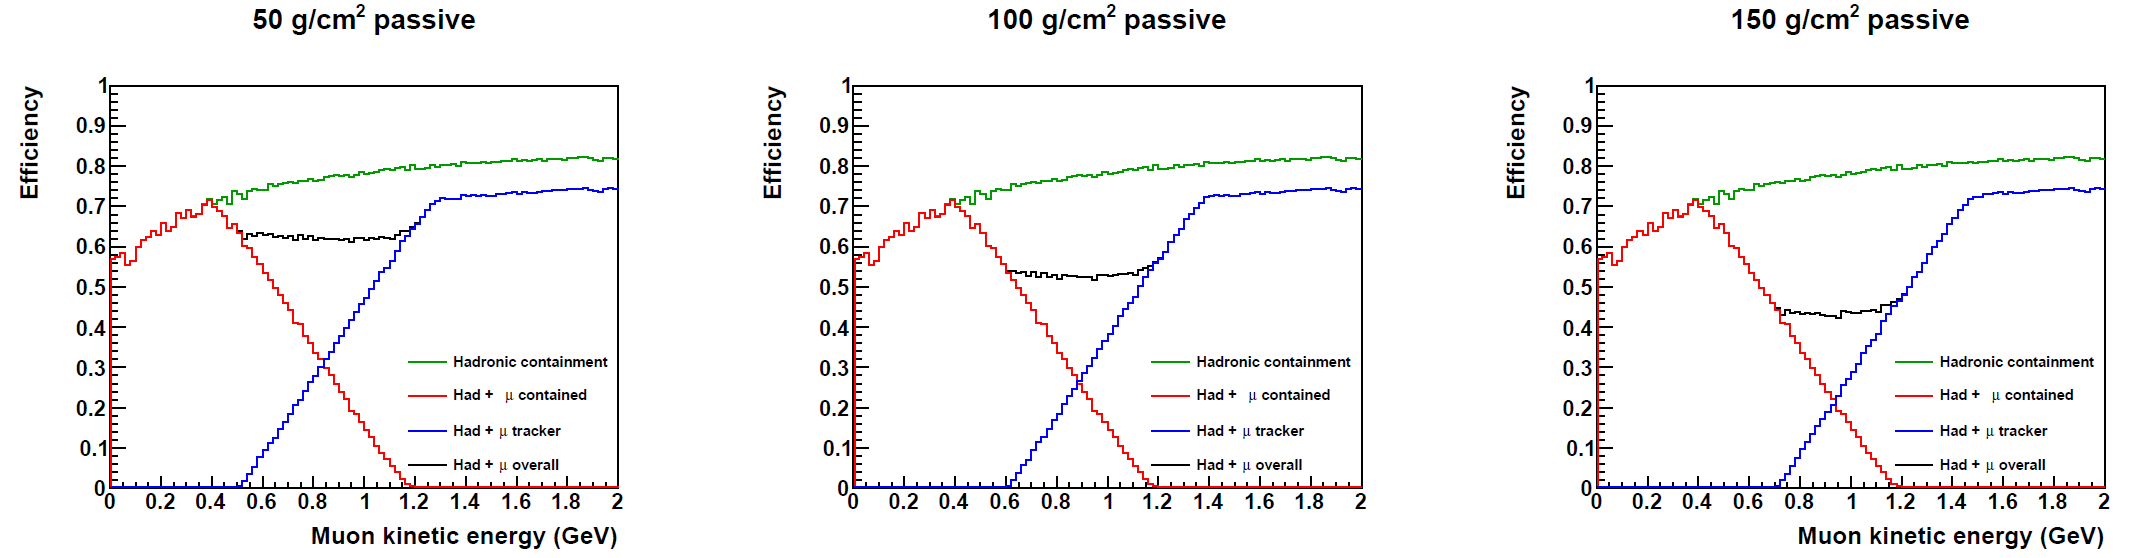
\includegraphics[width=0.95\textwidth]{graphics/cryostat/numu_cc_efficiency.png}
\end{dunefigure}

\subsubsubsection{Event reconstruction Requirements}
The required muon momentum resolution of the near detector is set by the momentum resolution achievable in the far detector. Oscillation parameters are inferred by comparing observed neutrino energy spectra in the FD to predictions. These predictions are constrained by ND data. If the energy resolution of the ND is worse than that of the FD, then theoretical models must be used to correct the predictions. Because of the nontrivial shape of the FD energy spectra (which is caused primarily by oscillations themselves), these corrections are sensitive not only to the detector model but also to neutrino interaction modeling. In order to extrapolate ND data to the FD without introducing additional modeling uncertainties, it is required that the ND energy resolution be equal or superior to that of the FD.

In the far detector (FD), muon momentum is reconstructed either by range or by multiple coulomb scattering (MCS). For muon momentum between 0.5 and 5 GeV, the resolution is 4\% by range and 15\% by curvature. Due to the large size of FD modules, the majority of muons will be reconstructed by range; a 2.5 GeV muon travels approximately 10 m in liquid argon and will be contained in a single FD module $\sim 80\%$ of the time. The resolution for reconstruction by range is used as the requirement for the ND. This 4\% is relatively at as a function of true momentum in the oscillation region. 

Muons that stop in the ND-LAr active region will be reconstructed by range in liquid argon. Muons will also be reconstructed primarily by range when they exit the ND-LAr detector and enter the temporary muon spectrometer (TMS), or the calorimeter of the ND-GAr detector. The ND-LAr active volume is 5 m long in the direction nearly parallel to the neutrino beam. To reject front-entering events, the most upstream 50 cm is excluded from analysis. To contain hadronic showers, the downstream 150 cm is also excluded. Some neutrino interactions produce minimal hadronic activity and can be analyzed when they occur within those 150 cm, but this is not possible in general, and attempting to analyze all interactions in this volume would introduce large uncertainties due to interaction modeling. Therefore we select CC $\nu_\mu$ events in a 300 cm region between 50 cm and 350 cm from the upstream face of the active volume. This means that for muons in the forward direction, the maximum path length in LAr is 450 cm, corresponding to a maximum muon kinetic energy of about 1.1 GeV. Above that energy, forward muons are never contained and must always be matched to tracks in the downstream spectrometer.

For 1 GeV muons, the 4\% resolution requirement means that the kinetic energy from range must be known to ~ 40 MeV, which corresponds to an upper bound of ~ 20 g/cm2 on the material traversed. If the uncertainty on the stopping point of the muon is greater than that, the momentum resolution will be dominated by that uncertainty rather than by fluctuations in ionization. For the inactive material in between the detectors, this 20 g/cm2 is not possible, so we instead exclude from analysis muons which exit the active LAr but do not enter the spectrometer. This exclusion causes a dip in the ND acceptance as a function of muon energy, which is shown in Figure \ref{fig:eff_numucc}. The dip is broadened by the fact that we can analyze interaction vertices over a 300cm region in ND-LAr, so muons that stop in the passive material have between 400 and 1100 MeV kinetic energy depending on the location of the vertex. The total thickness of passive material determines the minimum energy where tracker-matched muons begin to turn on. The fraction of muons which fall into the dip is related to the ratio of the total passive material thickness to the total thickness of the fiducial volume, which is 420 g/cm2.

\begin{dunefigure}[Muon reconstruction efficiency vs. q0,q3,Enu=2.0-2.5 GeV]{fig:eff_numucc_q0q3_2025GeV}
{Left: the efficiency for $\nu_\mu$ charged-current events in the ND-LAr fiducial volume to have a well-reconstructed muon and hadronic system, shown as a function of three-momentum and energy transfer to the nuclear system for $2.0 < E_\nu < 2.5\;\mbox{GeV}$ for 100 $\mbox{g}/\mbox{cm}^2$ passive material. Right: The ratio of the efficiency with 150 $\mbox{g}/\mbox{cm}^2$ passive material to 100 $\mbox{g}/\mbox{cm}^2$.}
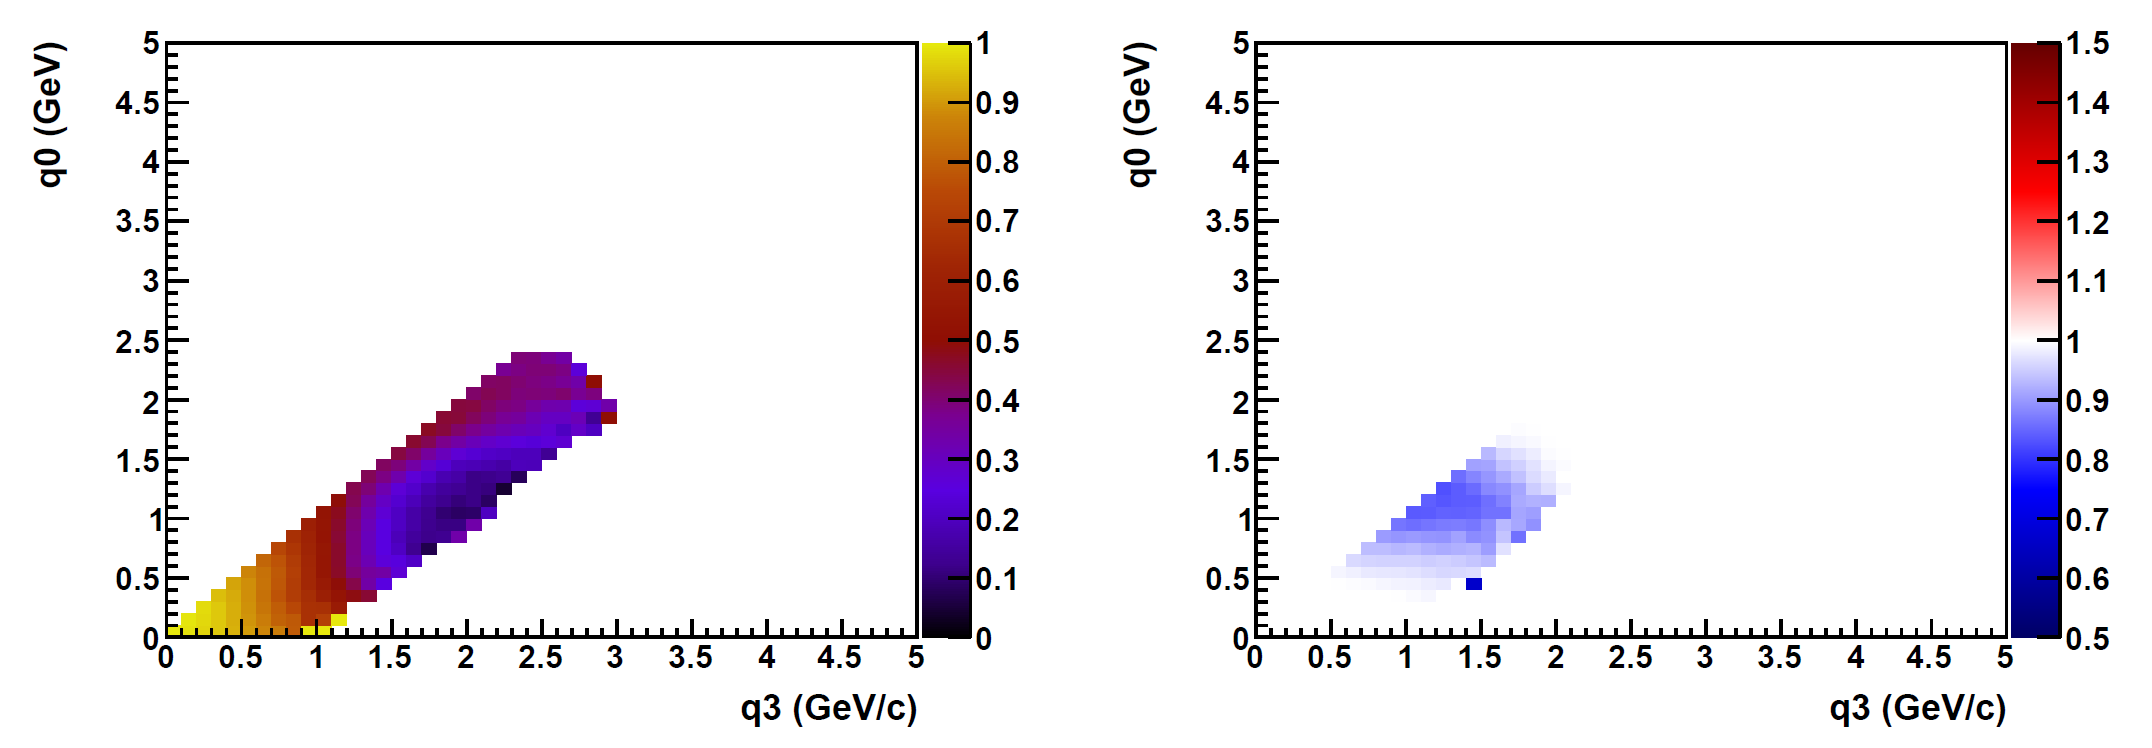
\includegraphics[width=0.95\textwidth]{graphics/cryostat/numu_cc_efficiency_q0q3_2.0-2.5GeV.png}
\end{dunefigure}

\begin{dunefigure}[Muon reconstruction efficiency vs. q0,q3, Enu=3.5-4.0 GeV]{fig:eff_numucc_q0q3_3540GeV}
{Left: the efficiency for $\nu_\mu$ charged-current events in the ND-LAr fiducial volume to have a well-reconstructed muon and hadronic system, shown as a function of three-momentum and energy transfer to the nuclear system for $3.5 < E_\nu < 4.0\;\mbox{GeV}$ for 100 $\mbox{g}/\mbox{cm}^2$ passive material. Right: The ratio of the efficiency with 150 $\mbox{g}/\mbox{cm}^2$ passive material to 100 $\mbox{g}/\mbox{cm}^2$.}
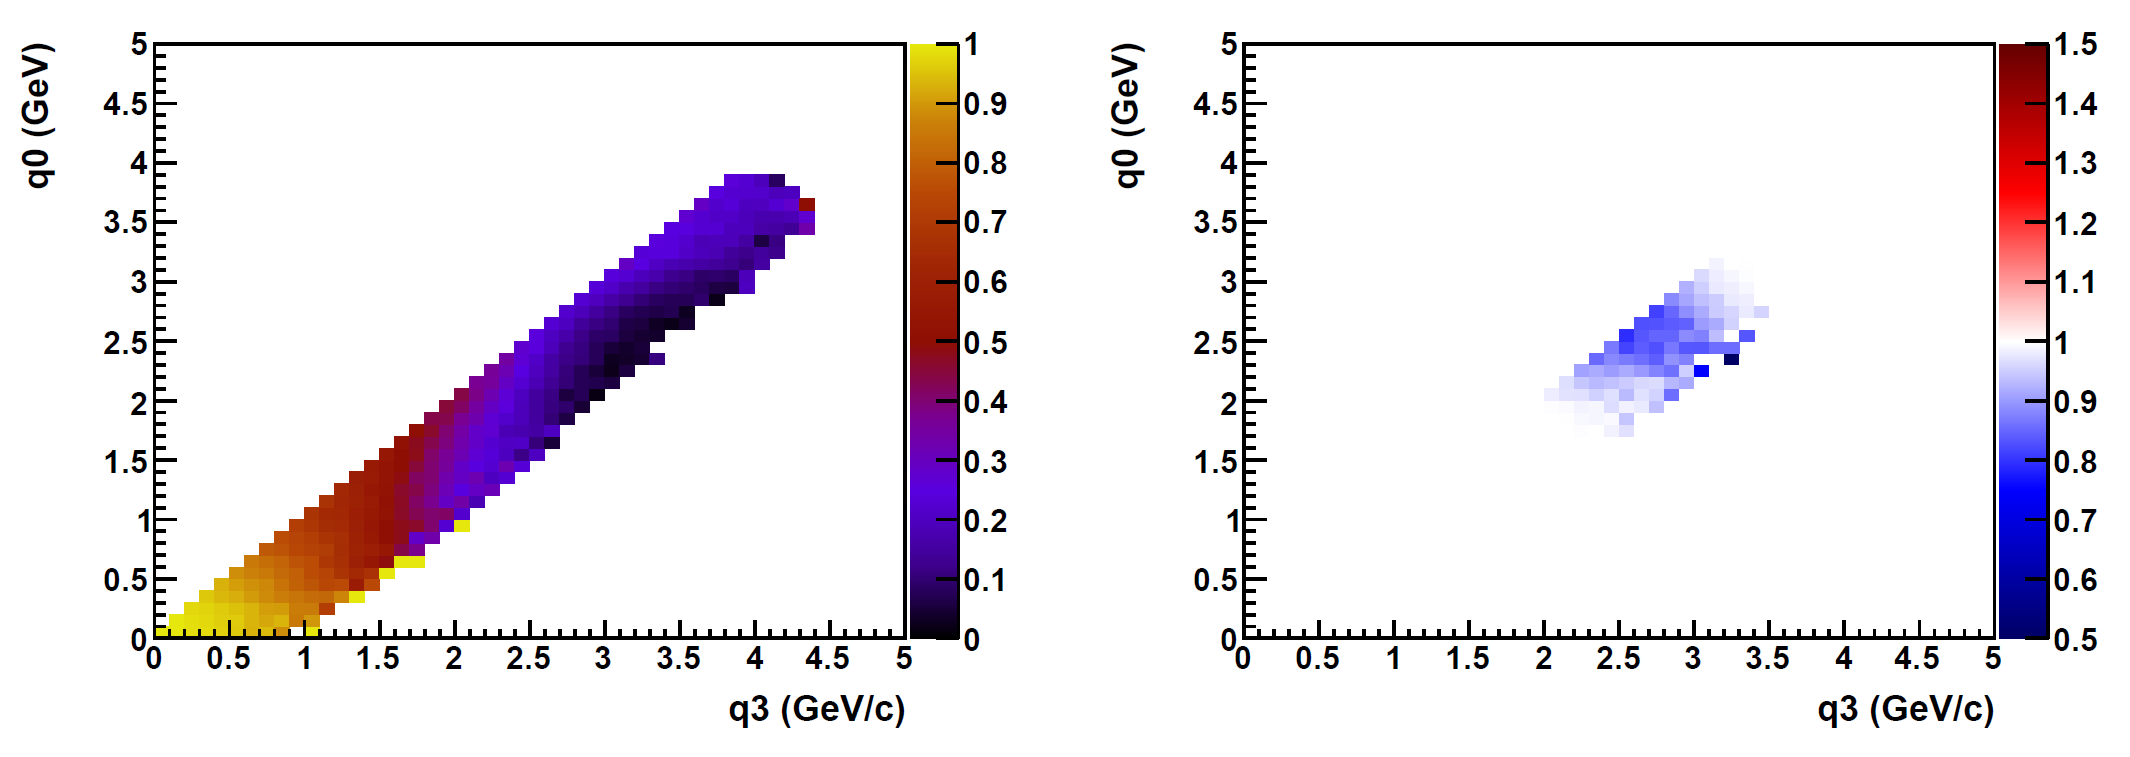
\includegraphics[width=0.95\textwidth]{graphics/cryostat/numu_cc_efficiency_q0q3_3.5-4.0GeV.png}
\end{dunefigure}

\begin{dunefigure}[Fraction of total cross section with less than 10\% efficiency]{fig:eff_numucc_10pct}
{The fraction of the total cross section in a region of $q_0-q_3$ space with efficiency below 10\%, as a function of neutrino energy. This is essentially the size of the black regions in Figures \ref{fig:eff_numucc_q0q3_2025GeV} and \ref{fig:eff_numucc_q0q3_3540GeV}, weighted by the total cross section.}
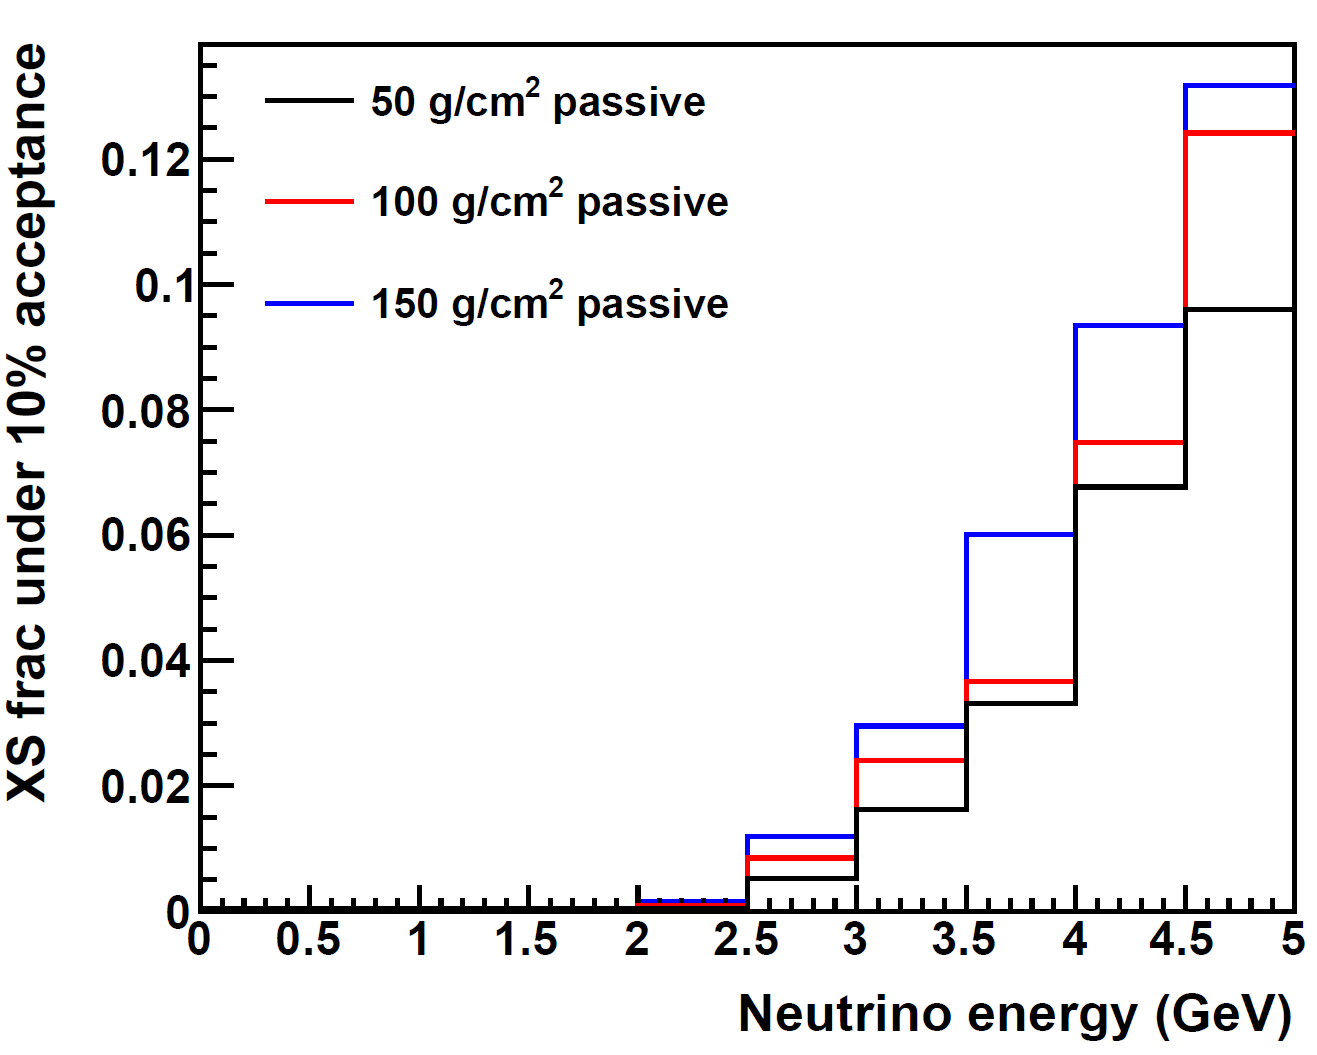
\includegraphics[width=0.65\textwidth]{graphics/cryostat/numu_cc_efficiency_10pct.png}
\end{dunefigure}


\subsubsubsection{Cryostat Wall Thickness}
Muon acceptance is defined as either stopping in the ND-LAr active volume, or penetrating into the active volume of the downstream spectrometer (TMS or ECAL). Starting at muon kinetic energy of 0.4, forward muons in the most downstream region of the fiducial volume begin to exit the active LAr. For muons of a given kinetic energy between 0.4 and about 1.2 GeV, there is essentially a dead region in the LAr fiducial volume, where tracks originating in this region will terminate in the passive material and their momenta cannot be measured at the required precision. The width of this dead region is proportional to (and exactly equal to, for muons that are exactly 6° above the neutrino beam) the total areal density of the passive material between the two detectors. As muon energy loss is proportional to the areal density traversed (measured in g/cm2), it is the integrated density along a straight-line trajectory connecting the two active volumes that impacts the physics. The electromagnetic radiation length and nuclear interaction length of the material in this region is irrelevant, because our physics analyses will not require tracking electrons or hadrons through this region.

The impact of the passive material on both muon and hadron reconstruction can be seen by looking at the efficiency to reconstruct both the muon and hadronic system as a function of energy transfer from the neutrino to the hadronic system, $q_0$, and three-momentum transfer, $q_3$. Neutrino interaction modeling issues map well onto this kinematic space; for full coverage of the neutrino cross section, it is critical that there not be any regions in this space where the ND efficiency is very low. For a given neutrino energy, $E_\nu$, the muon energy is related to the total hadronic energy $E_{had} = q_0$ by $E_\mu = E_\nu - q_0$. The muon angle is exactly forward when $q_0 = q_3$. Figure \ref{fig:eff_numucc_q0q3_2025GeV} shows the efficiency in this space for $2.0 < E_\nu < 2.5$ GeV and 100 g/cm2 total passive material, along with the relative change in the efficiency in increasing the passive material from 100 to 150 g/cm2. It is observed that losses are most significant in the forward region, as expected. Figure \ref{fig:eff_numucc_q0q3_3540GeV} shows the same thing for higher neutrino energy, $3.5 < E_\nu < 4.0$ GeV on the falling edge of the flux peak.


Regions of phase space with efficiency below 10\% are especially problematic. This typically means events can be reconstructed only in a very particular location within the detector, or only when the hadronic shower happens to be composed of certain final-state particles. In the DUNE-PRISM analysis, the method of using ND data itself to translate and rotate vertices in order to determine the efficiency correction with minimal dependence on interaction modeling breaks down when regions of phase space have such low acceptance. As such, we want to limit the fraction of the overall cross section as a function of neutrino energy that falls in the problematic regions. Figure 2.4 shows the fraction of the total cross section with total efficiency less than 10%.

Three main factors, which are closely related, drive the requirement of 100 g/cm2 total passive material. First, the desire to be able to directly constrain the modeling of the hadronic shower by measuring the same events in different regions of the detector. With less than 100 g/cm2, we are guaranteed for every muon energy at least a 1 m region in the upstream half of the fiducial volume where the muon is contained and the hadronic shower efficiency is high, and at least a 1 m region in the downstream half of the fiducial volume where the muon angular acceptance is high. Second, the fraction of the cross section in kinematic regions of low acceptance is less than 3\% up to 4 GeV neutrino energy as can be seen in Figure 4. This limits the events that have to be corrected with models instead of data. Third, the magnitude of the dip seen in Figure 2.2 is less than 30\%, which means a correction with an uncertainty of 10\% will lead to a total uncertainty on the extrapolated rate in this regime of less than 3\%.

It should be noted that there is physics benefit to exceeding the 100 g/cm2 requirement, and effort should be made to do so if it is possible without increasing cost. The impact on physics is continuous as a function of the passive material thickness, but generally it can be mitigated by the procedures described above up to 100 g/cm2. Increasing from 100 g/cm2 to 150 g/cm2 carries some physics risk, especially if the nuclear model and composition of the hadronic final states in the GENIE model is not correct, since these models are used as the baseline in this study. Above 150 g/cm2 there is a significant hole in the reconstruction. If the 100 g/cm2 requirement cannot be met for the entire downstream face of the LAr active region, it is better to use thick support beams over a small fraction of the downstream face as described below.

The physics requirement is on the total passive material, including passive LAr downstream of the active volume, the cryostat support structure, and cryostat insulation, and also including passive elements upstream of the active region of the muon spectrometer. The spectrometer passive elements are different in the ND-GAr system and TMS, and the ND-LAr system must functionally couple to either. The solenoid with partial return yoke in the reference design of ND-GAr has a 10 cm aluminum coil that is at least 37 cm of passive material. The requirement for the ND-LAr cryostat system is thus 60 g/cm2, with a target of 50 g/cm2 to allow for additional margin in the ND-GAr magnet design, which is not yet finalized.

\begin{dunefigure}[RMS deflection due to multiple scattering]{fig:mu_multiscat_rms}
{The expected RMS of the transverse deflection due to muon multiple scattering in the LAr cryostat is shown for different combinations of thicknesses of the uninstrumented LAr and the steel outer membrane. Due to its position upstream of the insulating foam, which results in a long lever arm, scattering in the LAr is more impactful than scattering in the outer membrane.}
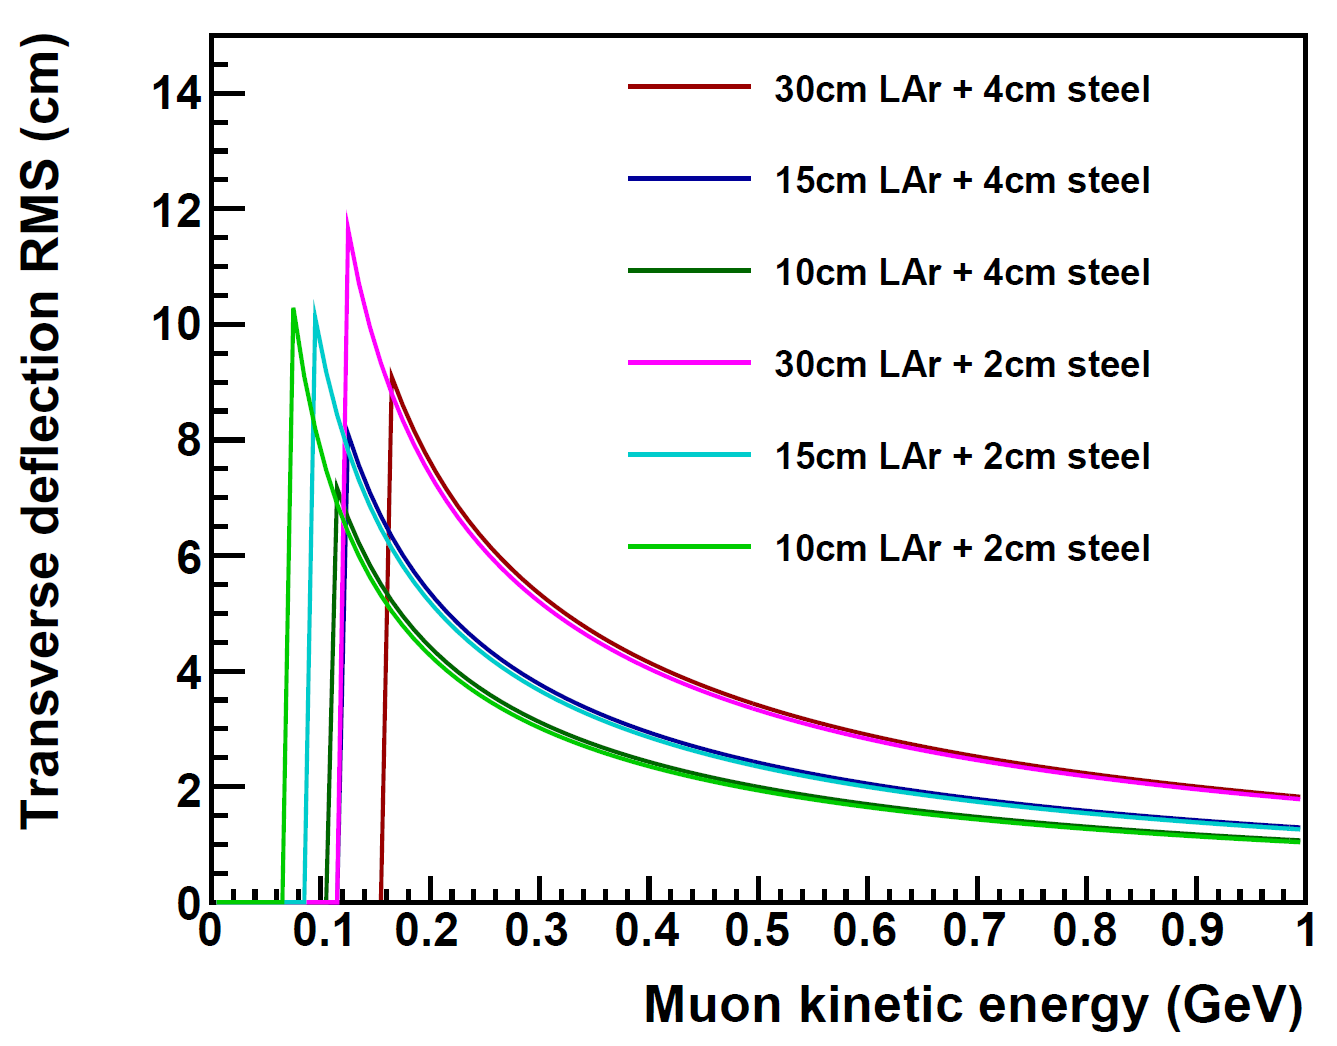
\includegraphics[width=0.65\textwidth]{graphics/cryostat/mu_multiscat_rms.png}
\end{dunefigure}

\begin{dunefigure}[Fraction of total cross section with less than 10\% efficiency compared to ProtoDUNE]{fig:eff_numucc_10pct_protodune}
{The uniform cryostat walls in Figure 4 are compared to a scenario with 100 $\mbox{g}/\mbox{cm}^2$ total for thin regions, but where only 16\% of the downstream wall area is more than 10 cm away from any steel beam in a ProtoDUNE-like cryostat.}
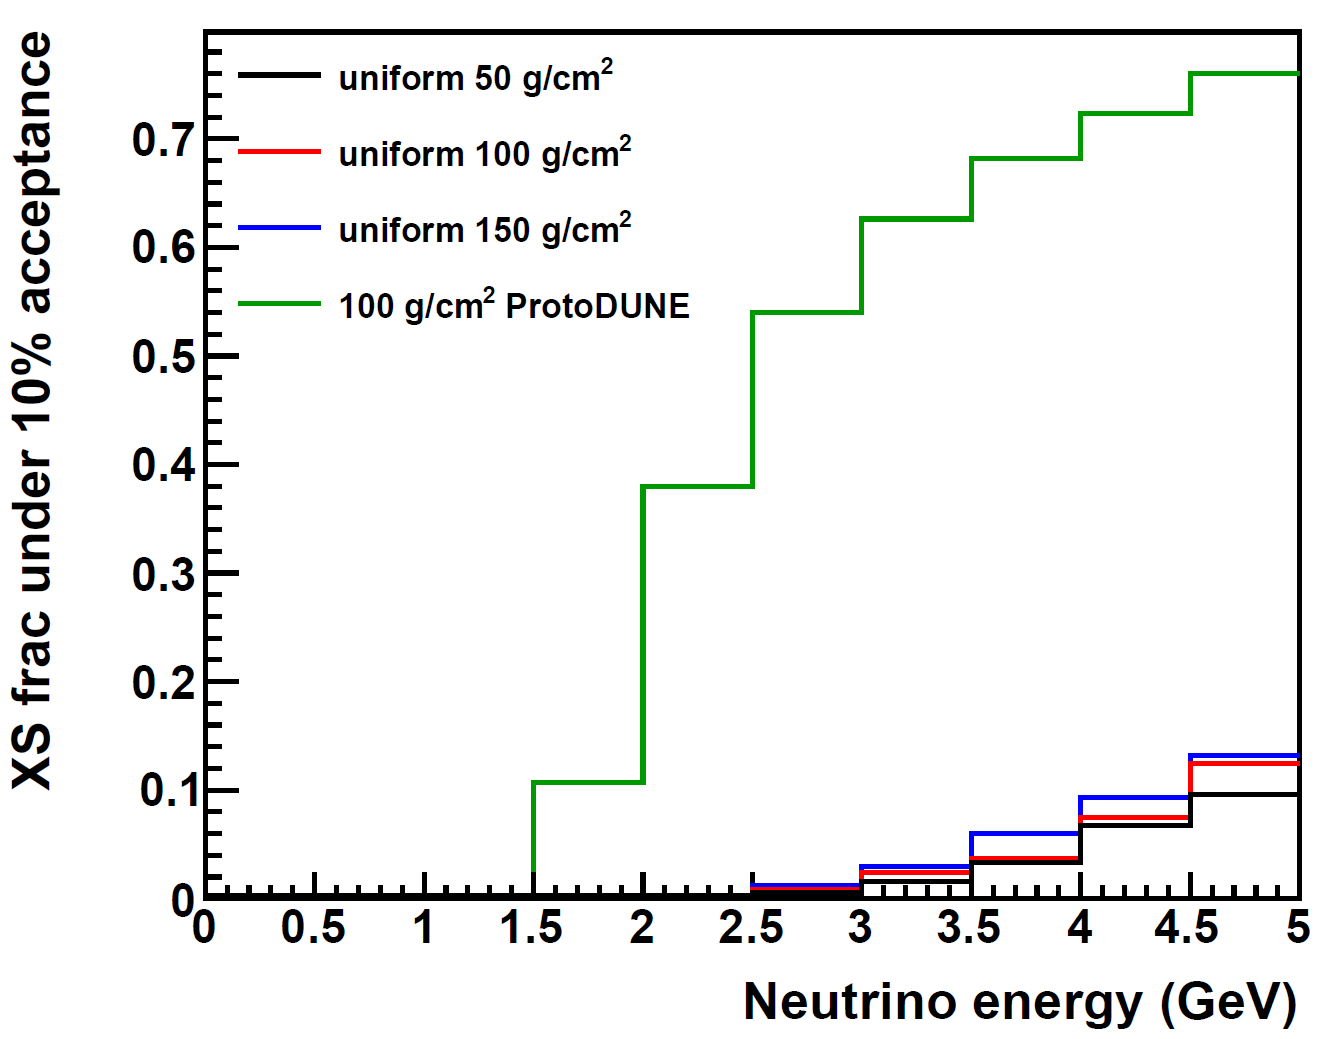
\includegraphics[width=0.65\textwidth]{graphics/cryostat/numu__cc_efficiency_10pct_protodune.png}
\end{dunefigure}


\subsubsubsection{Cryostat Wall Unifomity}
In addition to being sufficiently thin to preserve high-acceptance regions for CC $\nu_\mu$ interactions, the energy loss in the cryostat wall must be modeled, so that it can be added back to the energy estimate for tracks that are matched to the spectrometer. This places a requirement on the uniformity of the cryostat wall; if the wall is non-uniform, then it will introduce a smearing on this piece of the correction that may worsen the muon energy resolution beyond the requirement. The lowest momentum muons that will be analyzed by matching tracks to the spectrometer are about 600 MeV. This number assumes the maximum allowed passive material, and includes the 150 cm traversed in liquid argon. That muon will lose about 200 MeV in the passive material, about 100 MeV of which is in the ND-LAr passive material including the cryostat wall. We use the 4\% momentum resolution requirement to define a maximum uncertainty on the energy loss in the passive material of 24 MeV for a 600 MeV muon. Half of that would come from the ND-LAr cryostat and other passive material, or 12 MeV. Compared to a 50 g/cm2 thickness, that is a uniformity requirement of 12\% across the downstream face of the detector.

\subsubsubsection{Adding Support Beams}
We can tolerate higher nonuniformity if it is confined to a relatively small fraction of the overall 7 X 3 m active area. For example, a 10 cm wide steel support running down the middle of the downstream face of the cryostat could be mitigated in analysis by simply excluding muons that pass through it with minimal loss of physics coverage. The areal density integrated along a straight-line trajectory connecting the two active detectors is then irrelevant because the muons will be rejected anyway. If the 60 g/cm2 requirement cannot be met with a uniform cryostat wall, it is preferable to add support beams over a small fraction of the wall area, while keeping the majority of the area below 60 g/cm2, see Figure \ref{fig:eff_numucc_10pct}.

In this scenario, muons that pass very near the dense support structures will be excluded from analysis. It is critical that we are able to correct the muon energy for losses event by event, which will not be possible for muons that pass very near the dense regions as small deviations in their position will lead to large changes in energy loss. Due to multiple scattering in the passive material itself, a buffer around the beams is required. Uninstrumented LAr on the cold side of the cryostat is especially important, because small angular deflections there are amplified by the long lever arm of the insulating foam. Figure \ref{fig:mu_multiscat_rms} shows the expected RMS of the transverse deflection at the face of the spectrometer due to muon multiple scattering in the LAr cryostat. It assumes some uninstrumetned LAr, followed by a 2 mm stainless steel inner membrane, 80 cm of polyurethane insulating foam, and a steel outer membrane, followed by a 10 cm air gap. Muon energy loss is accounted for, and the turn-off at low energy in each configuration is due to muons that range out in the cryostat.

A 10 cm buffer around any beams is sufficient to account for multiple scattering, except possibly at very low muon energy. For a cryostat wall with many steel beams like the SBND or ProtoDUNE designs, this results in a significant loss of events. To cut at least 10 cm away from all beams and stiffeners creates four ~20 X 20 cm2 squares in every 1 X 1 m2 of total area, resulting in a reduction factor of 16\%. Applying that to the acceptance, the fraction of the cross section phase space with very low acceptance below 10\% is much higher than for a uniform wall, as shown in Figure \ref{fig:eff_numucc_10pct_protodune}.

This loss in acceptance could be mitigated in two ways. First, effort should be made to increase the spacing between beams. A steel outer membrane of a few cm with larger beam spacing could create significantly larger square regions in between beams where events would be accepted. Second, these squares could be instrumented outside the outer membrane, to potentially tag muons that do not intersect beams. This may allow a reduction in the 10 cm buffer around the beams to account for multiple scattering if the non-beam-traversing events can be efficiently tagged. The feasibility of this should be further studied with simulation.

These vertical beams will create acceptance differences as a function of the horizontal position of the event, which corresponds to the off-axis position in the PRISM analysis. The flux changes as a function of off-axis position become significant at the 50cm level, so the width of any single support should be less than half of that, or 25 cm. The total width of the supports should not exceed 10\% of the area of the downstream face. The remaining 90\% of the area must meet the 12\% uniformity requirement. The position resolution will be degraded by the presence of passive argon between the active region and the cryostat wall, so it will not be possible to exclude muons that pass through the supports event by event if the gaps between the supports are too small. For that reason, there should be as few support beams as possible while meeting the other requirements stated above.


%\subsubsection{Infrastructure and Tooling}
%\subsubsection{Auxiliary Pieces and Installation}

%%%%%%%%%%%%%%% one subsec for each wbs element
\subsection{Membrane Cryostat Safety}
\label{sec:cryost-des-safety}

The \dword{ndlar} cryostat has to comply with the Fermilab Environment, Safety and Health Manual (FESHM). Chapter 5031.7 of the FESHM defines the procedure for the design, fabrication, erection, quality control, testing, maintenance, repair, and operation of membrane cryostats and the relevant requirements [1]. The metallic membrane is not a structural component of the system and has a containment function only. The design of the membrane is done following EN14620 [8].

The external warm structure provides support for all internal and external loads acting on the cryostat. The structure (steel frame and composite window) will be designed and verified following the International Building Code [x]. A memorandum of understanding [x] was prepared and approved by the Fermilab Safety Committee. The structural support can be verified using the American Institute for Steel Construction Standard ANSI/AISC 360 [2]. The design of the warm supporting structure is performed per the European standard for steel structure design and construction EN1993 [3], which is equivalent to the U.S. ANSI/AISC 360 [4]. The main design technique is based on the Finite Element Analysis (FEA) method. The design approach is to generate detailed FEA models of the vessel and to perform a detailed stress analysis of each component. 

The \dword{ndlar} cryostat structure design is independently verified by a U.S. professional structural engineer.
A final verification and certification (where applicable) of the documentation related to examinations, inspections of materials, in-process fabrications, and acceptance tests are performed at the end of the project by the same professional engineer.


%%%%%%%%%%%%%%% one subsec for each wbs element
\subsection{Warm Structure}
\label{sec:cryost-des-warm}
The steel warm structure is constructed from wide flange I-beams that are welded into wall/floor structures and then bolted together; these provide mechanical support to both the cold membrane and insulation.  The 10mm steel skin is welded to the I-beams, as well as adjacent skins to form a vapor barrier.  This external steel structure provides the mechanical support required against the liquid argon hydrostatic load, argon-gas overpressure load, gravitational loads, and external constraints. The design intent is to provide a support surface flatness for the membrane cryostat within +/- 5mm.
The warm structure base interfaces to a steel beam platform, which itself interfaces to a linear rail-system for translating the entire structure along the length of the underground cavern.
The warm structure’s leak integrity is be verified prior to cold structure installation.  Qualification activities may include, but are not limited to, the following:
\begin{enumerate}
    \item Dye Penetrant Analysis
    \item Helium Leak Rate Measurement 
\end{enumerate}
Responsibility for qualification of the warm structure rests with LBNL and the DUNE-ND Project.

%Subsection for warm structure design
\subsubsection{Warm Structure Design Description}
\label{sec:cryost-des-warm-design}

\begin{dunefigure}[\dword{ndlar} cryostat warm structure]{fig:cryostat}
{Exterior warm beam structure of \dword{ndlar} cryostat.}
\includegraphics[width=0.95\textwidth]{graphics/cryostat/cryostat.png}
\end{dunefigure}

The \dword{ndlar} cryostat warm structure, shown in Figure \ref{fig:cryostat}, consists of a continuous 10mm thick steel vapor barrier backed by a structural frame of steel columns and beams. The vapor barrier protects the insulation from ambient condensation and allows for a dry gas purge of the insulation volume. The vapor barrier is not required or expected to provide tertiary liquid argon containment. On one side of the cryostat, a composite window replaces the steel structure in order to limit the impact on crossing muons. The window is connected to the steel beams with scarf joints, described later.

The structure is subjected to three main loads: the liquid argon hydrostatic load; the overpressure load; and the gravity acceleration. The Argon has a density of 1400 kg/m3, and the level height assumed is 4.5 m with respect to the membrane floor. The overpressure load is assumed to be equal to 350 mbar. This load is conservative with respect to the requirements provided by the FESHM [1]. The safety relief valve will be dimensioned accordingly. Additional loads that will have to be considered in future are the earthquake loads and the potential sloshing of the liquid during the motion of the cryostat. For the moment these loads were neglected, as they are not fundamental in the evaluation of the structural performances (serviceability), which is the main purpose of this preliminary analysis.

The steel structure design relies heavily on the past work performed on similar cryostats (protoDUNE, LBNF). The beams and columns are made of steel H-beams. In the preliminary design presented here, the spaces between beams and and columns are reinforced with smaller H-beams (see Figure \ref{fig:cryostat}). Presently, corrugations are being considered in place of the smaller frame. Local deformation analyses showed that with this design it would be possible to obtain similar local deflections, whilst improving significantly the production process.

\subsubsection{Composite Window Design}
\label{sec:cryost-des-composite}

The composite window tries to minimize the impact on the crossing muons.  The window is very large, covering an area of approximately \SI{8}{\m} X \SI{8}{\m}. The final dimensions of the window can still change depending on the area assigned to the detector array. A composite design can significantly improve the performances in this respect when compared to steel. The window will have to react to the hydrostatic and overpressure loads applied by the \dword{lar} through the foam. Two typical design configurations are used for composite components of particle detectors: sandwich designs, or eccentrically stiffened designs. The sandwich construction is made of a central lightweight core, ‘sandwiched’ between two layers of fiber reinforced plastics. In general, the cored construction can provide better performances for distributed loads and is then advantageous for these hydrostatic loads. The design of a cored plate needs the definition of the following parameters:skin material, core material, skin thickness, core thickness.

\begin{dunefigure}[Mechanical performances of core materials]{fig:cryostat-coregraphs}
{Mechanical performances of typical core materials as a function of the core density.}
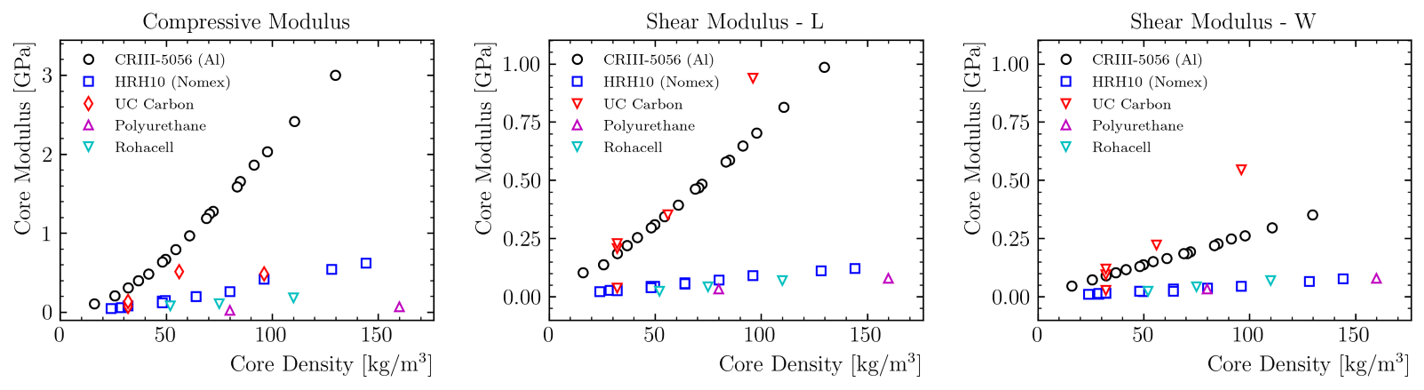
\includegraphics[width=0.95\textwidth]{graphics/cryostat/cryostat-coregraphs.png}
\end{dunefigure}

\begin{dunefigure}[Shear modulus of selected polyurethane]{fig:cryostat-polyu}
{Shear modulus of the selected polyurethane as a function of its density.}
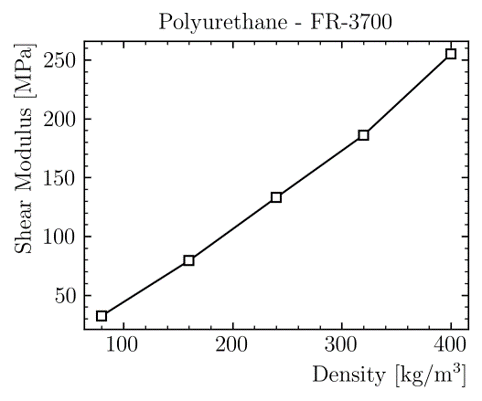
\includegraphics[width=0.65\textwidth]{graphics/cryostat/cryostat-polyu.png}
\end{dunefigure}

A comparison of the mechanical performances of typical core materials, as a function of the core density, is shown in Figure \ref{fig:cryostat-coregraphs}. Most materials have comparable performances, with the exception of aluminum and carbon based cores. These, however, have a significantly higher cost associated. Polyurethane was selected as core material. The fire resistant series FR-3700 is being considered at the moment. The variation of its shear modulus as a function of its density is shown in Figure \ref{fig:cryostat-polyu}. Two possible fiber materials were identified for the external layers: carbon and glass. Regarding the sizing of the plate, to maximize the final mechanical performances a thickness of 372 mm was selected, using all the space allowed by the detector envelope.

\begin{dunefigure}[Composite window parametric optimization]{fig:cryostat-coreoptimize}
{Results from the parametric optimization of the composite window design.}
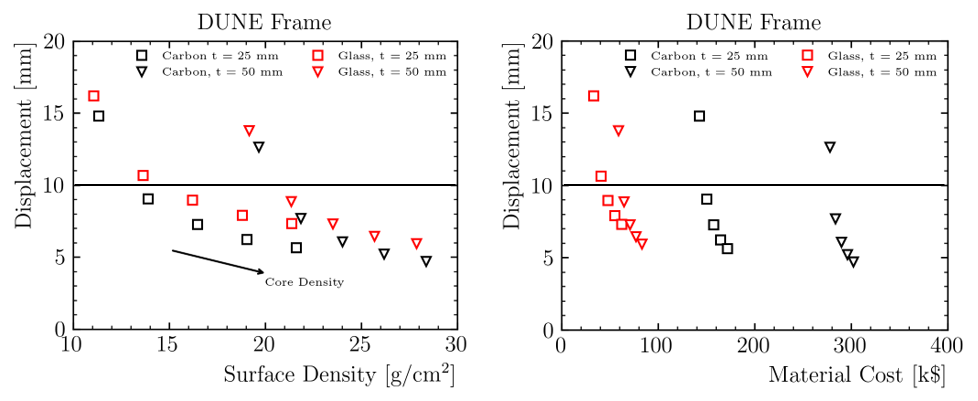
\includegraphics[width=0.95\textwidth]{graphics/cryostat/cryostat-coreoptimize.png}
\end{dunefigure}

An optimization study was performed in order to determine the best parameters for the core density and the thickness of the reinforced plastic layers. Two thickness were considered for the latter: 25 mm and 50 mm. The results of the optimization are shown in Figure \ref{fig:cryostat-coreoptimize}; the plots show the maximum displacement at the plate, as a function of the surface density and material cost. The surface density is the main index used to evaluate the impact of the plate on the crossing particles. The displacements of the plate were computed in a FE model of the whole cryostat. Further details on the modelling approach are reported later in this section. The results suggest that the carbon fiber solution has small advantages on performance but significantly higher costs.

\begin{dunefigure}[Surface density as a function of the material cost]{fig:cryostat-surfdencost}
{Surface density as a function of the material cost for different acceptable designs of the composite window (displacement lower than 10 mm).}
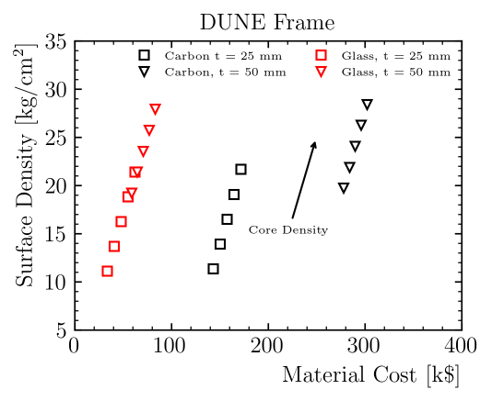
\includegraphics[width=0.65\textwidth]{graphics/cryostat/cryostat-surfdencost.png}
\end{dunefigure}

A displacement threshold of 10 mm was defined to accept or reject the different designs. This allows to select fewer acceptable designs, shown in Figure \ref{fig:cryostat-surfdencost}. The best solutions are obtained using glass fiber while minimizing the mass: this is a consequence of the fact that already with 25 mm thick glass fiber skins is possible to obtain the required performances. The selected core density is 400 g/m3. 

%Insert Table - ARL

Table 2.x provides the contribution to the overall surface density of the different layers crossed by the muons. The total expected surface density is 66 g/cm2. About 60\% of this value is due to the LAr. About 10\% is then provided by the steel membrane and the polyurethane insulation. The composite window provides 16\% of the total surface density. The table also provides the surface density that the steel frame would provide if used instead of the composite window. The average surface density, obtained by spreading uniformly the amount of steel over the whole window, would be equal to 40.8 g/cm2, 2.5 times the one of the composite window. The advantage is even more apparent when considering the material that the muons would cross while travelling through one of the steel beams: the surface density in this case is equal to 260 g/cm2, which is 16 times the value provided by the sandwich design.

\subsubsection{Window Joint Design}
\label{sec:cryost-des-window}

\begin{dunefigure}[Composite window to steel frame scarf joint design]{fig:cryostat-scarf}
{Composite window to steel frame scarf joint design.}
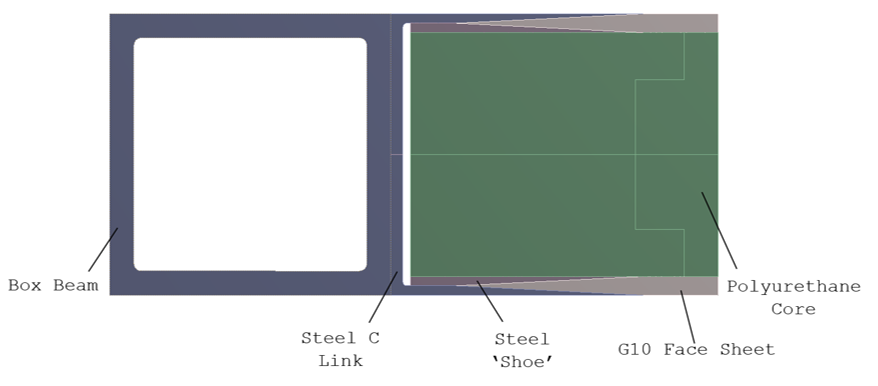
\includegraphics[width=0.95\textwidth]{graphics/cryostat/cryostat-scarf.png}
\end{dunefigure}

The composite window has to be connected to the steel frame with a configuration that guarantees stiffness and strength to the whole system. Preliminary analyses were carried out considering simple configurations (single/double lap joints), revealing that these would not be able to guarantee the required stiffness and strength within a reasonable length. A scarf joint configuration was selected instead. This type of design can carry significantly higher load, with the associated burden of a more complex production process. The connection design is shown in Figure \ref{fig:cryostat-scarf}: a box beam surrounds the whole window, providing torsional and bending stiffness; steel ‘c-links’ and ‘shoes’ are welded to the beam; the face sheets are connected to these with two separate scarf joints. The design allows the use of a denser foam core near the window with respect to the one used in the rest of the window. The production process is shown in Figure \ref{fig:cryostat-scarfsteps}, and consists of the following steps:

\begin{dunefigure}[Window/frame joint production process]{fig:cryostat-scarfsteps}
{Window/frame joint production process.}
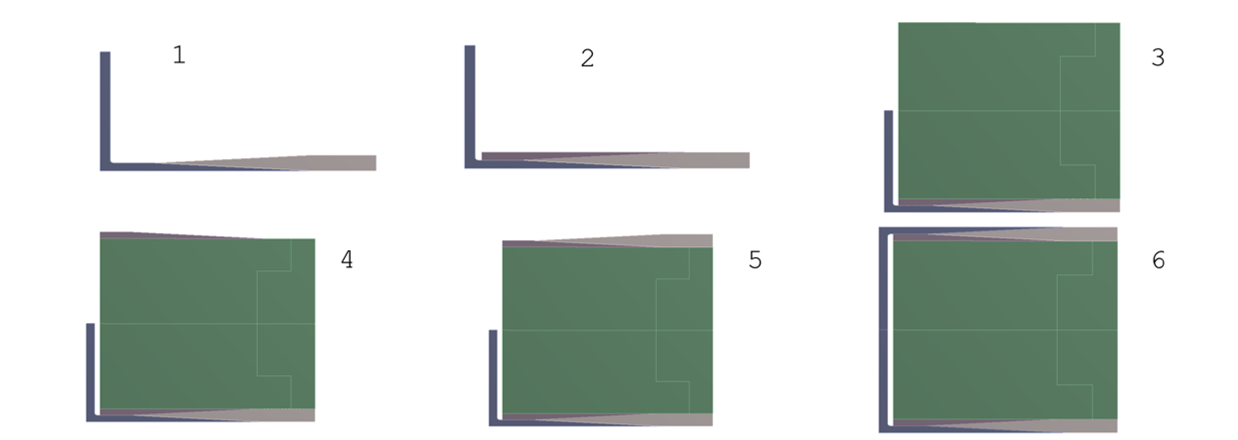
\includegraphics[width=0.95\textwidth]{graphics/cryostat/cryostat-scarfsteps.png}
\end{dunefigure}

\begin{enumerate}
\item Lay-up the bottom face sheet on the steel c-joint bottom half
\item Glue the bottom joint steel ‘shoe’
\item Glue the core
\item Glue the top joint steel shoe
\item Lay-up the top face sheet
\item Weld the c-joint, then weld to the box beam
\end{enumerate}

\subsubsection{Preliminary FE Analyses}
\label{sec:cryost-des-warm-FEA}

\begin{dunefigure}[FE model of the LAr cryostat]{fig:cryostat-fea-bc}
{FE model of the LAr cryostat: geometry (left), boundary conditions overview (right).}
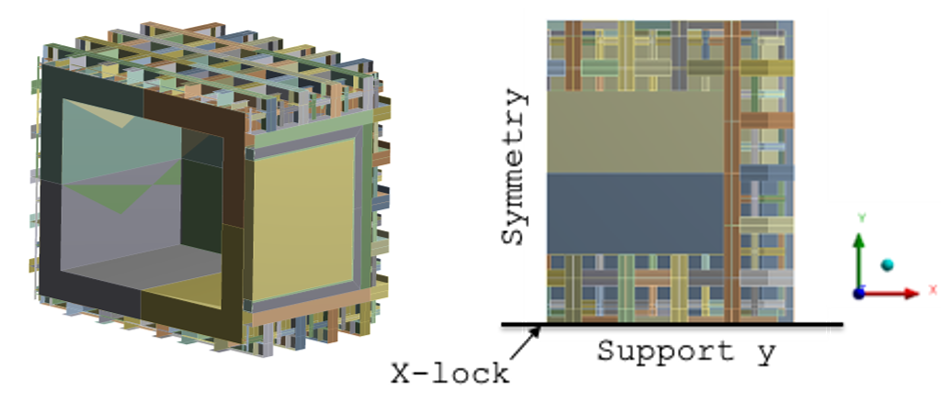
\includegraphics[width=0.75\textwidth]{graphics/cryostat/cryostat-fea-bc.png}
\end{dunefigure}

A preliminary FE analysis was performed in order to verify the mechanical performances of the structure. The geometry of the model is shown in Figure \ref{fig:cryostat-fea-bc}. The model is limited to half of the cryostat (YZ symmetry). The steel plates and the frame are represented by shell elements, and the composite plate and the polyurethane foam insulation by solid elements. All the elements were bonded together at their interfaces. The density of the foam was assumed to be 90 kg/m3. Mechanically, it was represented as an incompressible fluid with Young’s modulus of 10 MPa and a Poisson ratio close to 0.5.

The detector is simply supported by a rigid floor. Two different constraint conditions are considered: a bonded frictionless contact, not allowing separation but with sliding allowed in the floor plane, and non-linear frictionless contacts that allow separation. The central point of the detector is locked in the horizontal (x) direction. The following loads were applied:

\begin{enumerate}  
\item LAr hydrostatic load, with a density of 1400 kg/m3 and a liquid level height of 4.5 m with respect to the membrane floor
\item An overpressure load of 350 mbar
\item Gravitational acceleration
\end{enumerate}

\begin{dunefigure}[FE results]{fig:cryostat-fearesult}
{Deformation of the detector due to the gravitational load (a), hydrostatic pressure (b), overpressure (c), and with all the loads applied at the same time (d). These results were obtained fixing the bottom of the cryostat to the floor.}
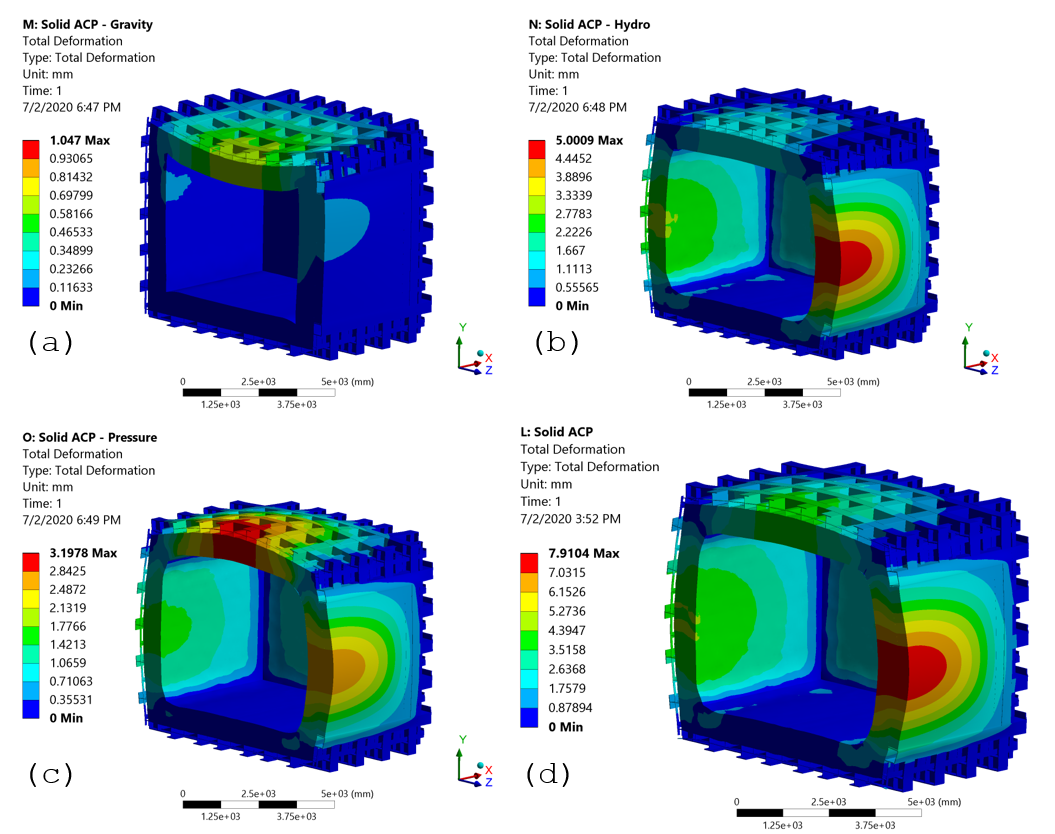
\includegraphics[width=0.75\textwidth]{graphics/cryostat/cryostat-fearesult.png}
\end{dunefigure}

\begin{dunefigure}[Normal displacement on a path]{fig:cryostat-displacementpath}
{Normal displacement on a path (shown on the left) passing along the middle plane of the composite plate.}
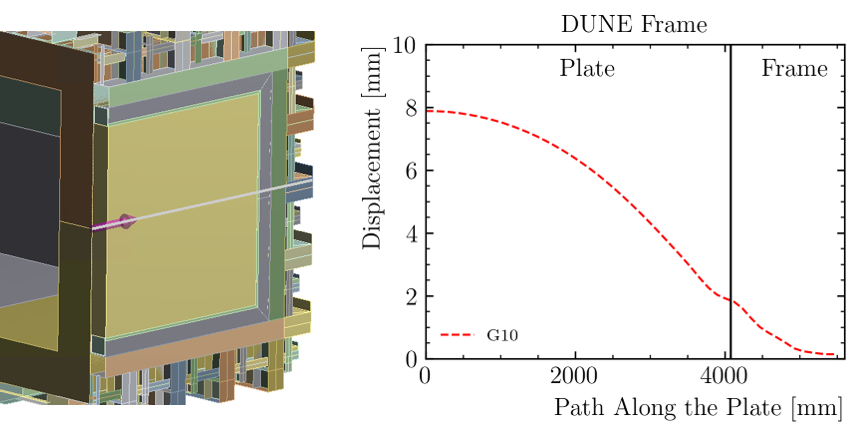
\includegraphics[width=0.75\textwidth]{graphics/cryostat/cryostat-displacementpath.png}
\end{dunefigure}

The model results are shown in Figure \ref{fig:cryostat-fearesult} for the no separation, sliding allowed case: the total deformation of the detector is equal to 7.9 mm. The gravity deflects the roof of 1 mm, with negligible impact on the deformation of the window; the hydrostatic pressure contributes for a 5 mm displacement on the window; the overpressure for 3.2 mm.

To obtain a reference value, the composite plate was tested in a simpler model with no frame and simple constraints at its border. When the middle plane of the plate was simply supported, the total displacement was equal to 7.9 mm under the same loads. Fixing also the rotations the total displacement is instead equal to 2.6 mm. This is the best possible value that this plate might reach in an infinitely rigid construction. In reality, the deformation of the constraint is significant, as shown in \ref{fig:cryostat-displacementpath}: the frame adds 2 mm of rigid motion to the plate because of its deformation at the support points, and another 3.3 mm because of their rotation.

\begin{dunefigure}[Stresses in the steel frame and plate]{fig:cryostat-framestress}
{Stresses in the steel frame (left) and in the composite plate (right).}
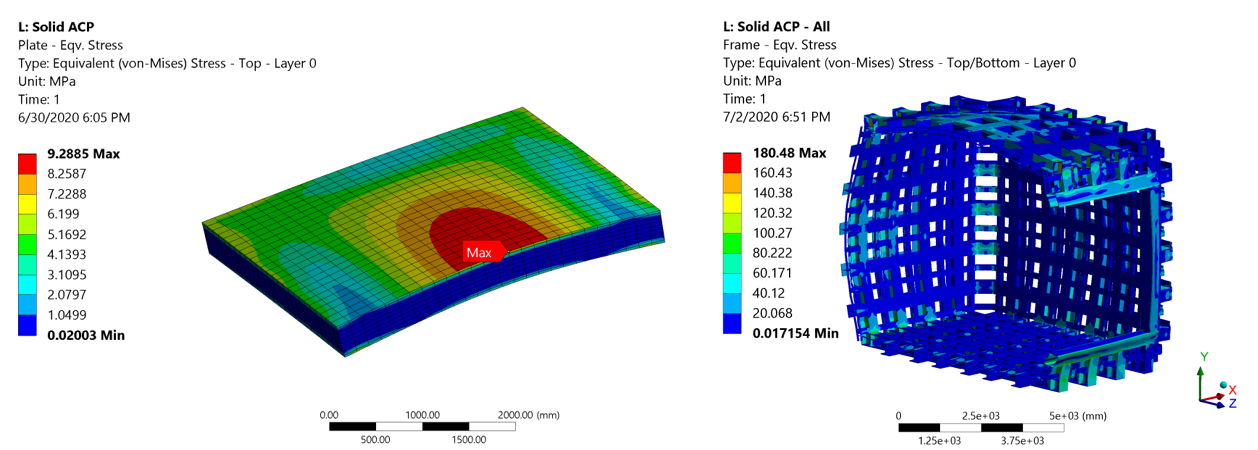
\includegraphics[width=0.75\textwidth]{graphics/cryostat/cryostat-framestress.png}
\end{dunefigure}

The stresses acting on the steel frame are shown in Figure \ref{fig:cryostat-framestress}, left. The maximum stress is 180 MPa on the square beam joint. This value might be reduced by adding local reinforcements in the most stressed regions, as was done for example in ProtoDUNE. The stresses applied to the composite plate are instead negligible (lower than 10 MPa), seen on the right in the Figure.

\begin{dunefigure}[Total deformation]{fig:cryostat-deform}
{Total deformation of the detector (left). Gap between the floor and the detector bottom side. These results are obtained allowing separation between the bottom of the cryostat and the ground.}
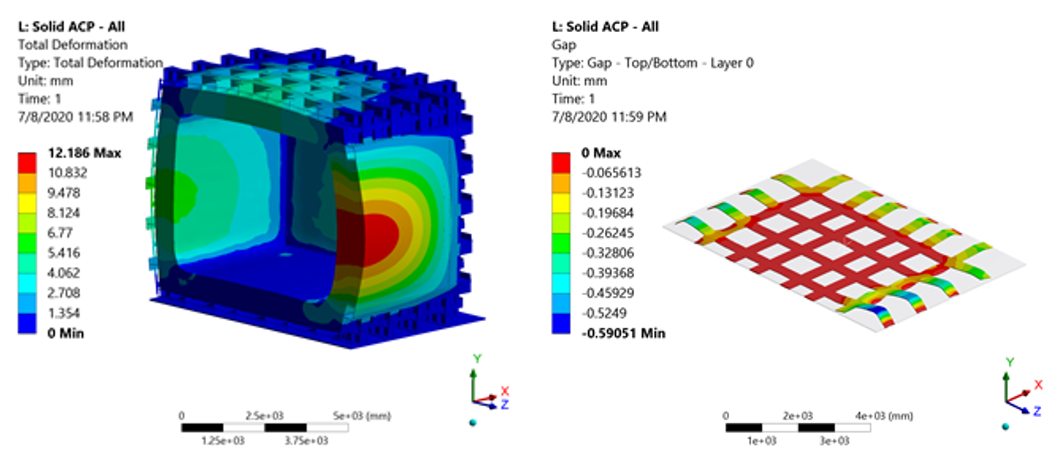
\includegraphics[width=0.75\textwidth]{graphics/cryostat/cryostat-deform.png}
\end{dunefigure}

The model results when allowing separation between the floor and the cryostat bottom are shown in Figure \ref{fig:cryostat-deform}: the total displacement on the window is higher and equal to 12.18 mm. There is some lifting close to the corners, with a maximum gap of 0.6 mm. This allows for some additional rotation of the corner, resulting in higher total displacements. Adding stiffeners in the corners that are experiencing lifting should bring the deformations closer to the values from the model with no separation allowed.

\subsubsection{Composite Window Joint Performances}
\label{sec:cryost-des-warm-joint}

The joint was designed with a progressive modelling strategy in mind:
\begin{enumerate}
\item 2D analysis to quickly optimize the geometry
\item Detailed analysis on a 3D model
\item Sub-model critical regions
\item Experimental verification
\end{enumerate}

Ideally, the process will be iterative, allowing to feed the experimental data back to the numerical analysis process. At this stage, no experimental verification was performed, and the performances were only analyzed via FE analysis.

\begin{dunefigure}[Total joint deformation and stress]{fig:cryostat-scarffea}
{Total deformation (left) and Von Mises equivalent stress (right) as computed in the plane stress model of the joint.}
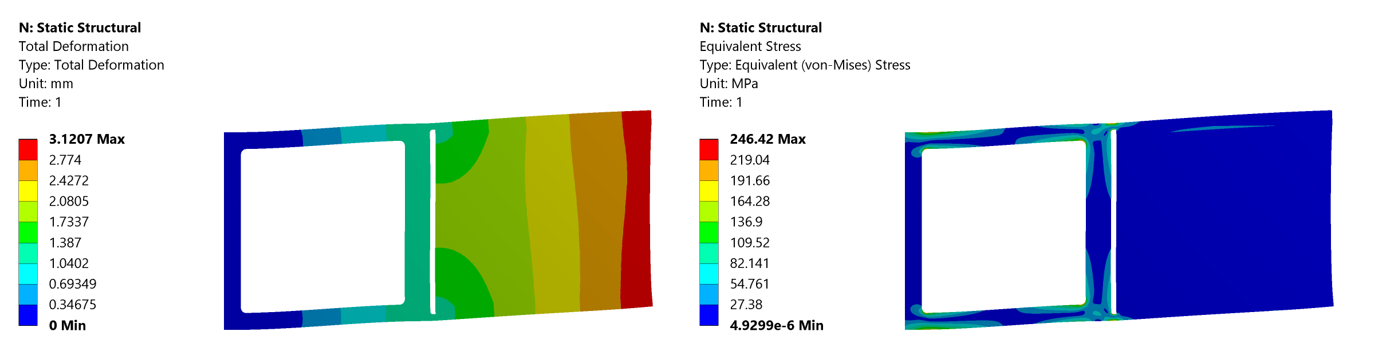
\includegraphics[width=0.95\textwidth]{graphics/cryostat/cryostat-scarffea.png}
\end{dunefigure}

\begin{dunefigure}[Scarf joint glue stress]{fig:cryostat-glue}
{Stress in the scarf joint glue: frictional stress (left) and normal stress (right).}
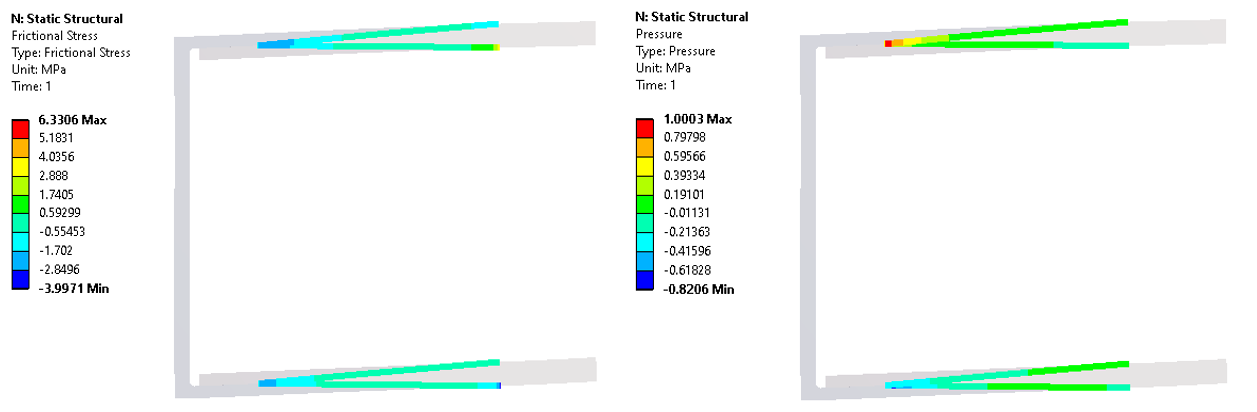
\includegraphics[width=0.95\textwidth]{graphics/cryostat/cryostat-glue.png}
\end{dunefigure}

The first model produced is a simple 2D model with plane stress elements. The model is shown in Figure \ref{fig:cryostat-scarffea}: the box beam was considered to be fixed at his left edge, and on the right edge of the model loads listed above were applied. This model allowed for a quick optimization of the joint geometry. The results from the selected joint geometry are shown in Figure \ref{fig:cryostat-scarffea}: the joint compliance is almost all the box beam constraint. This should guarantee similar results as the one obtained from the 3D analysis (the joint does not provide additional compliance). The computed stress in the composite components is negligible, while the stress in still is high in some corners. This might be reduced by adding some local reinforcements, or increasing the radiuses. Is also possible that a small amount of plastic deformation might be allowed in these corners. Finally, it is worth noticing that this is a very conservative load case where there is no longitudinal support for the plate (constrained only on 2 edges out of 4).

The stresses in the glue are shown in Figure \ref{fig:cryostat-glue}: the maximum frictional stress is equal to 6 MPa, while the maximum normal stress is equal 1 MPa. As a criteria, we consider that the maximum average shear stress allowed on the glued to is equal to 5 MPa, and the maximum tensile average equal to 10 MPa. The obtained values are more or less 1 order of magnitude lower than this criteria.

\begin{dunefigure}[Scarf joint submodel results]{fig:cryostat-joint-stress}
{Joint submodel: displacements applied on the contour of the submodel (left); frictional stress on the glue (centre); tensile stress on the glue (right).}
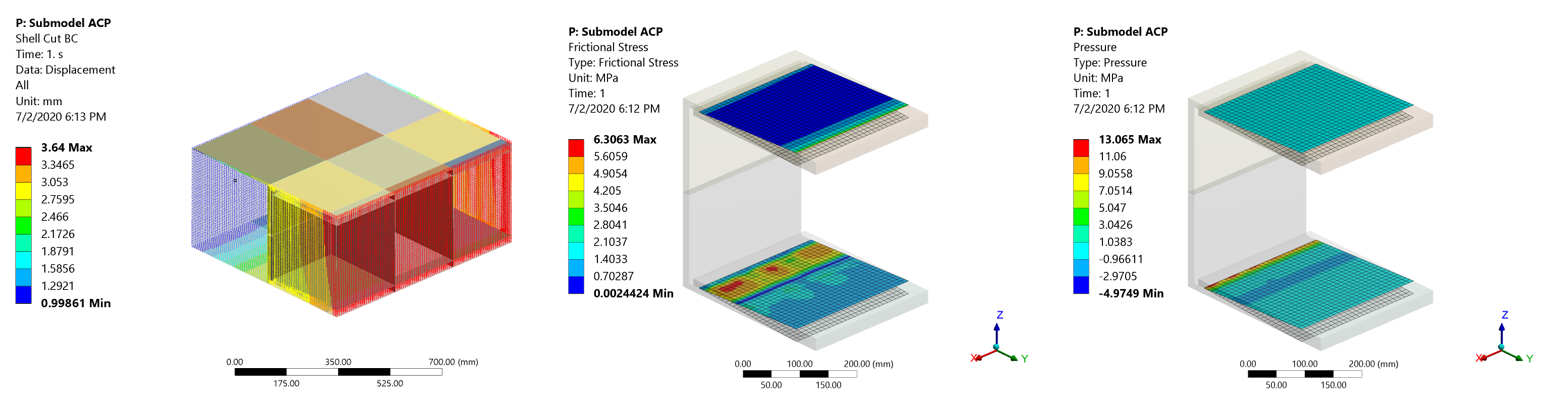
\includegraphics[width=0.95\textwidth]{graphics/cryostat/cryostat-joint-stress.png}
\end{dunefigure}

The joint was finally tested in the 3D model, and the critical regions were analysed with a refined submodel. The model geometry and the displacements applied on the submodel contour are shown in Figure \ref{fig:cryostat-joint-stress}. These displacements are interpolated from the global model and applied on the cut boundary. Computed stresses in the glue are also shown in Figure \ref{fig:cryostat-joint-stress}: the maximum frictional stress is 6 MPa, the maximum tensile stress is 5 MPa. Also in this case the criteria is satisfied with significant margin.

%%%%%%%%%%%%%%% one subsec for each wbs element
\subsection{Cold Structure}
\label{sec:cryost-des-cold}
The cold vessel design utilizes the stainless steel membrane containment technology as seen in Figure \ref{fig:protodune-mem}. The thermal insulation requirements necessitate a nominal insulation thickness equal to 800mm (an insulation thickness of 600mm would be desirable if the RHI requirement (<10 W/m2) can be satisfied).  The cold membrane and insulating structure provides both a primary and secondary membrane for two levels of liquid containment.  Liquid argon containment at the boundary of the warm steel structure is not required.  A 10mm thick, leak-tight steel skin is present behind the insulation and acts as a vapor barrier from the ambient environment and as an enclosure for circulated nitrogen gas.

\begin{dunefigure}[Cryostat cold structure membrane example]{fig:protodune-mem}
{Cryostat cold membrane example, ProtoDUNE cold membrane shown above.}
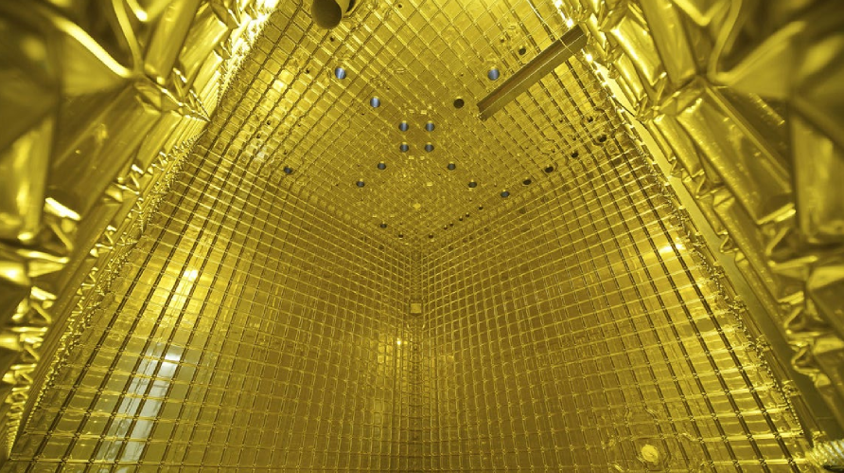
\includegraphics[width=0.75\textwidth]{graphics/cryostat/protodune-mem.png}
\end{dunefigure}

The general through-wall construction of the cold structure is shown in Figure \ref{fig:cryostat-coldstruc}.

\begin{dunefigure}[Cryostat cold structure membrane example]{fig:cryostat-coldstruc}
{Cryostat cold membrane through-wall construction.}
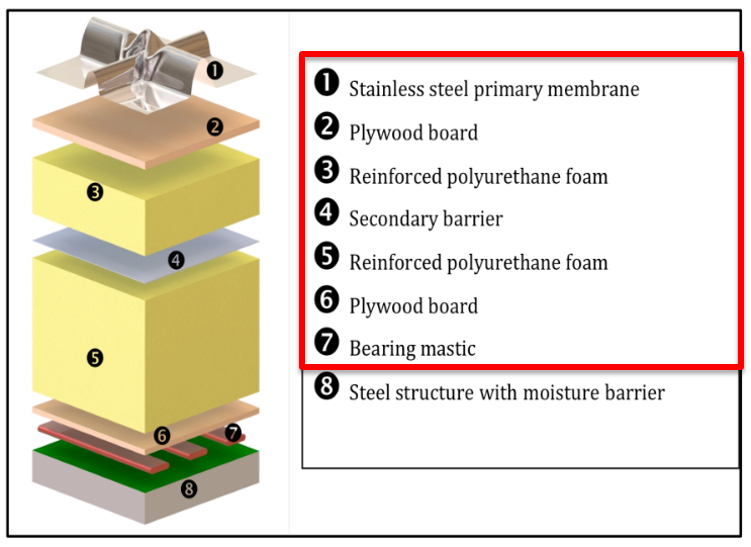
\includegraphics[width=0.65\textwidth]{graphics/cryostat/cryostat-coldstruc.png}
\end{dunefigure}


%%%%%%%%%%%%%%% one subsec for each wbs element
\subsection{Cryostat Lid}
\label{sec:cryost-des-lid}
The \dword{ndlar} cryostat lid is segmented into three main sections: cryogenic services, \dword{lartpc} module support and services, and pressure relief end section.  The cryogenics section is installed first and provides liquid and gaseous argon services to the main cryostat volume, as shown in Figure \ref{fig:cryostat-cryogenicslabels}.  This lid section consists of a liquid argon sprayer supply line with a gaseous argon return; gaseous argon make-up gas, momentum gas, piston purge and pressure control; cryostat liquid argon fill line; and gaseous argon evaporative boil off return line.  Additionally, the cryogenic lid section is equipped with feedthroughs for a pressure sensor, temperature driven level sensor, purity monitor, cold trap, and internal cameras and lighting.  Liquid supply lines are vacuum jacketed both in ambient environment and within the cryostat.  Gaseous return lines to the liquid argon condenser are also vacuum jacketed. 

\begin{dunefigure}[\dword{lartpc} section cryostat lid]{fig:cryostat-cryogenicslabels}
{\dword{lartpc} section cryostat lid section with detector array and services.}
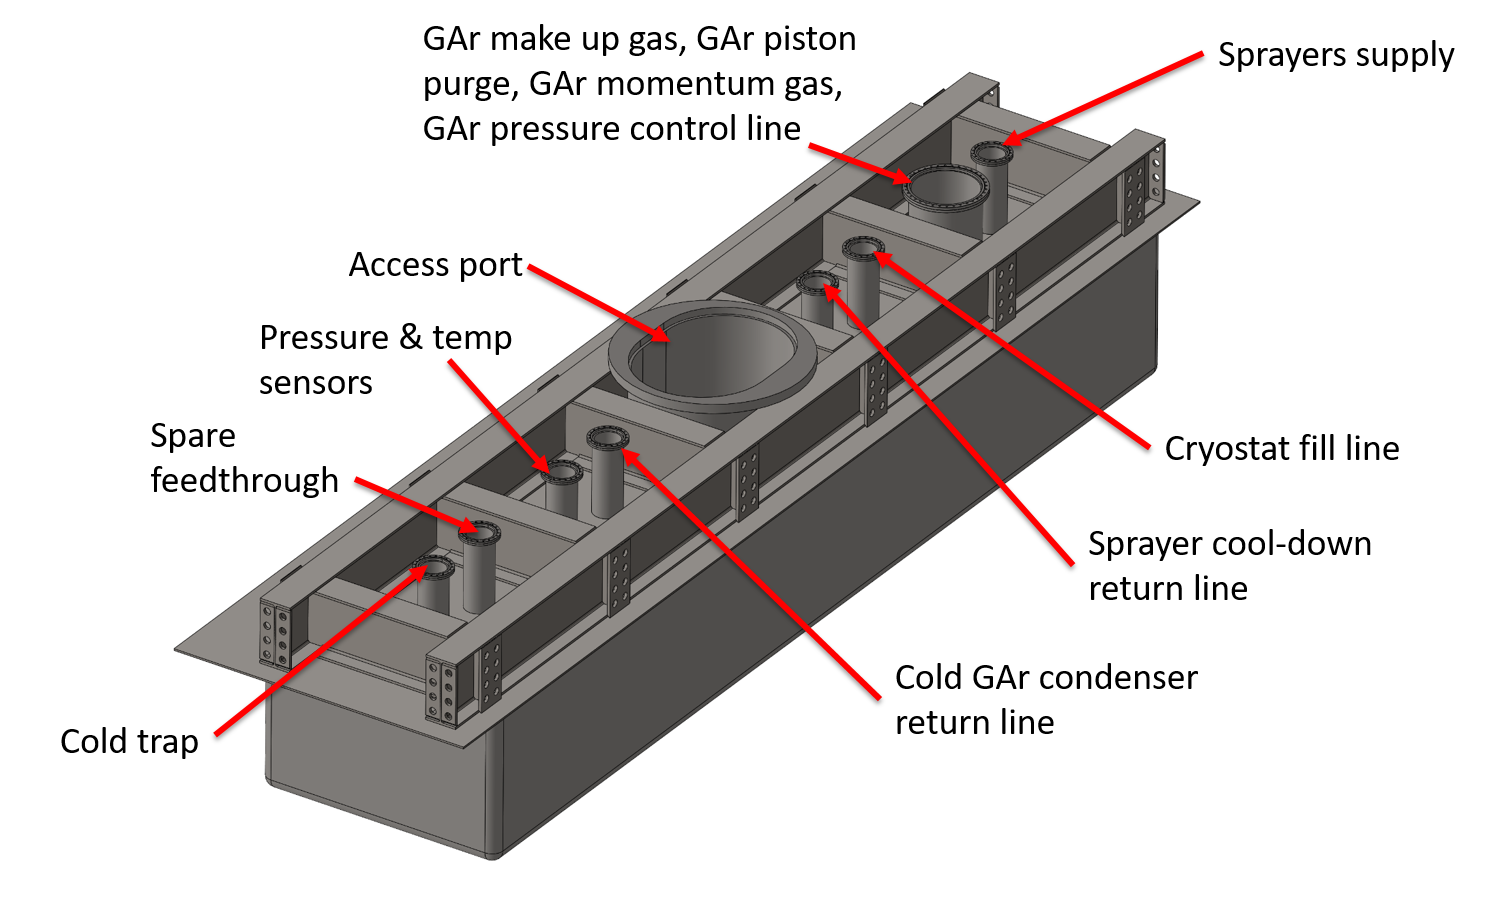
\includegraphics[width=0.65\textwidth]{graphics/cryostat/cryostat-cryogenicslidlabels.png}
\end{dunefigure}

The \dword{lartpc} sections provide mechanical support for the detector modules; as well as penetrations for detector subsystem services.   Each detector module has a dedicated feedthrough for its high voltage delivery and power/signal routing for the charge readout, light readout and calibration subsystems; this results in five identical penetrations through this lid section.  Additionally, at the end of the detector module row, purified liquid argon services are also fed through the cryostat lid.  The \dword{lartpc} lid section with detectors is shown in Figure \ref{fig:cryostat-TPClid}.

\begin{dunefigure}[\dword{lartpc} section cryostat lid]{fig:cryostat-TPClid}
{\dword{lartpc} section cryostat lid section with detector array and services.}
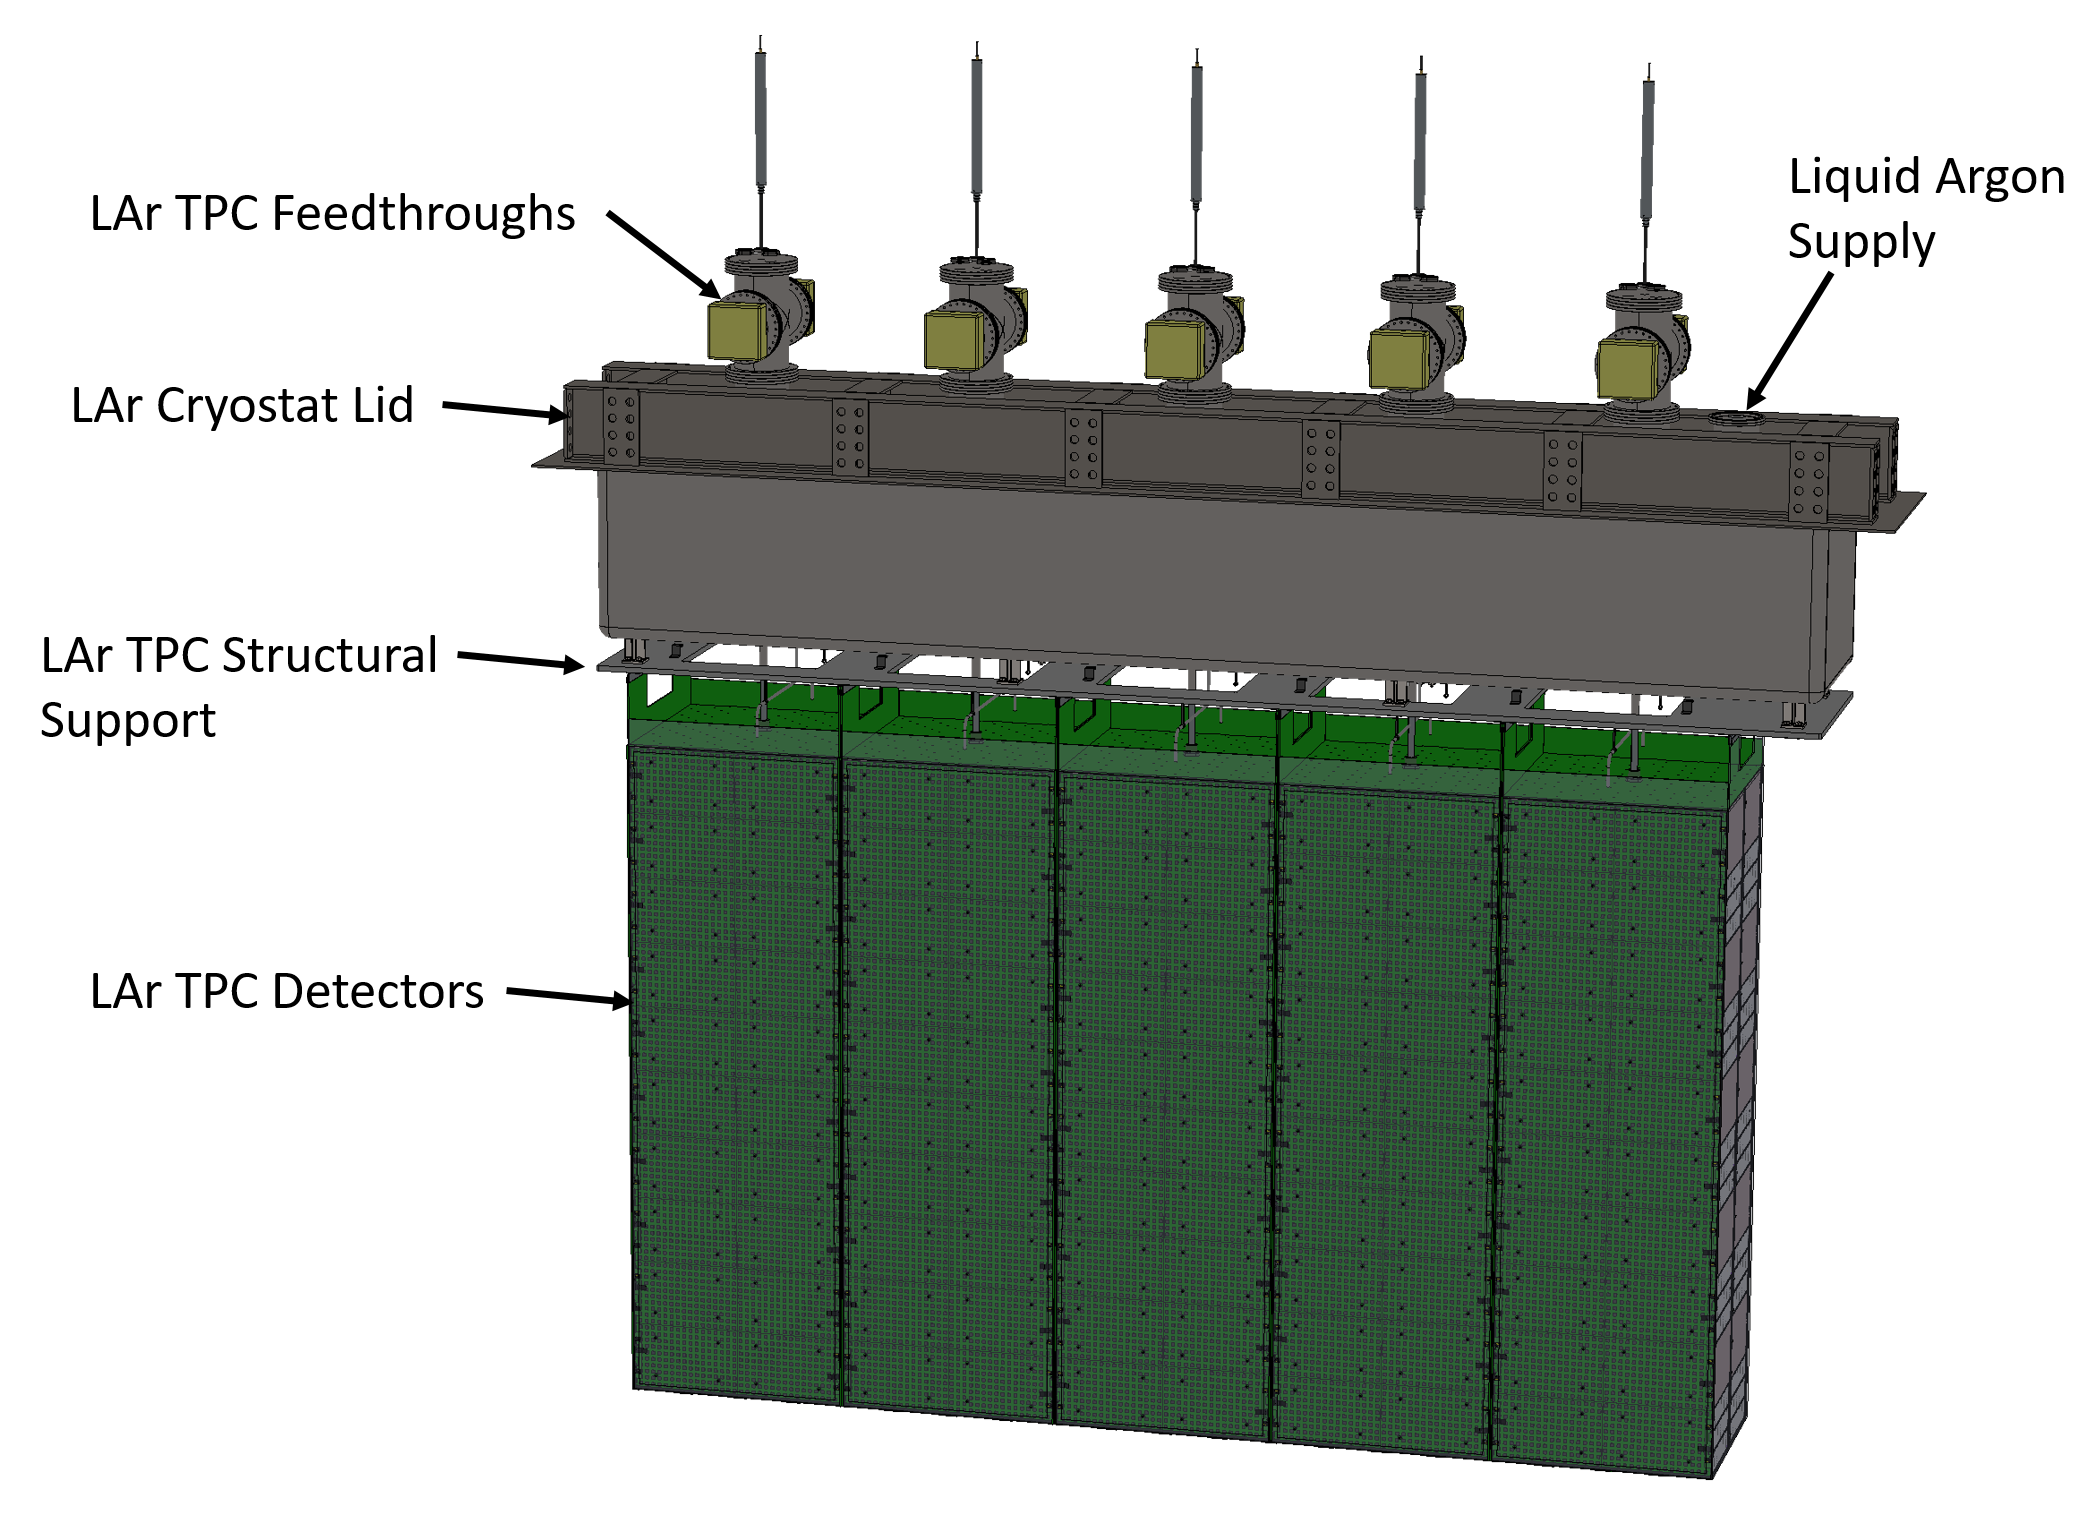
\includegraphics[width=0.65\textwidth]{graphics/cryostat/cryostat-TPClid.png}
\end{dunefigure}

The final lid section contains the cryostat pressure relief valve.  This section is also intended to be field machined to final dimensions to ensure proper fit.  Each cryostat lid section consists of a 10mm steel plate and beam structure, similar to the cryostat warm structure main body.  The top lid shall have a nominal insulation thickness of 800mm and an internal stainless steel cold membrane on the bottom surface; however it is not envisioned that this surface is corrugated.

\begin{dunefigure}[LAr cryostat services]{fig:cryostat-services}
{Liquid argon cryostat top lid services.}
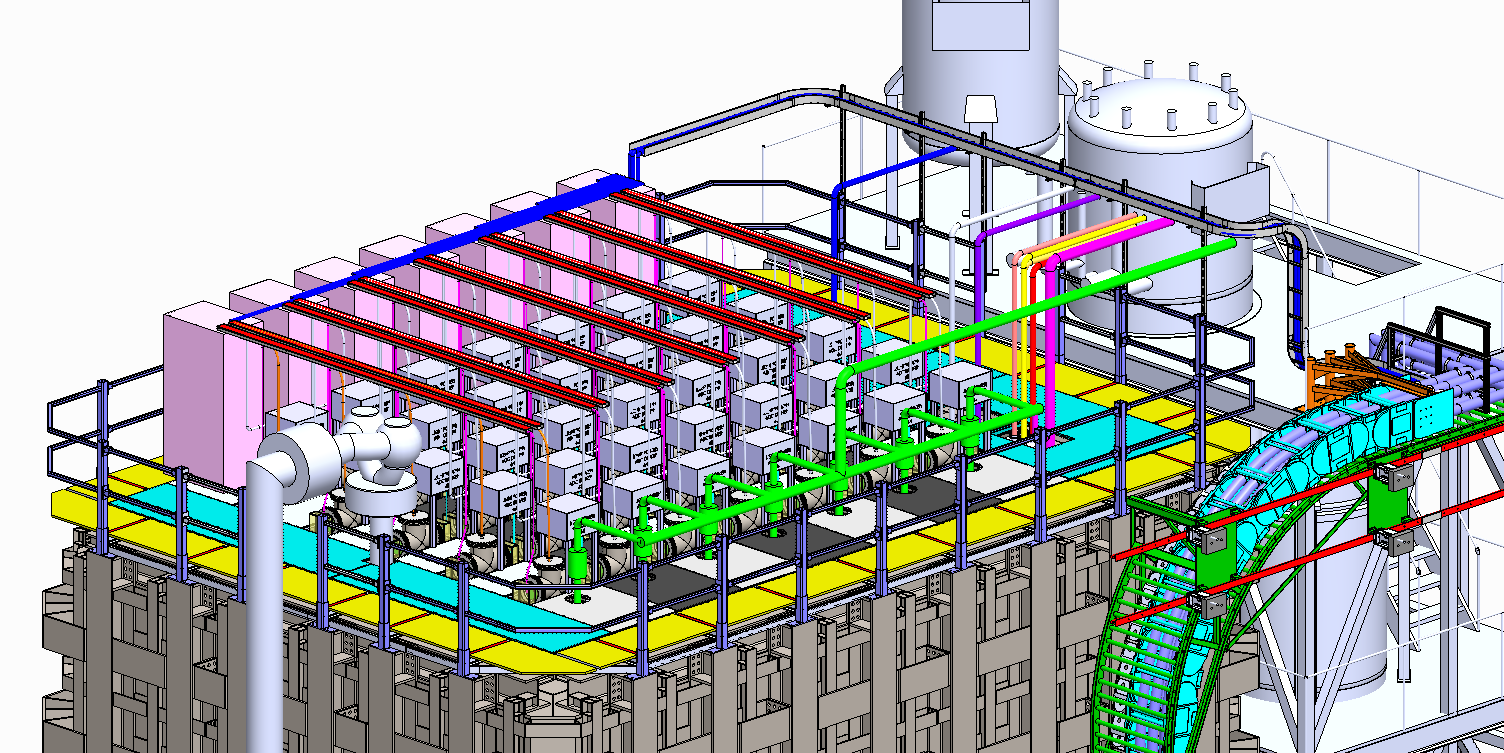
\includegraphics[width=0.95\textwidth]{graphics/cryostat/cryostat-services.png}
\end{dunefigure}

The warm side of the cryostat lid contains all of the required feedthrough ports for the charge readout, light readout, high voltage, and calibration subsystems.  Each module feedthrough has its power and signal cables route to local or row end electronics enclosures.  Module row cryogenics and cryostat bath cryogenics services are also routed on the top lid of the cryostat.  Electrical and cryogenic services on the cryostat top lid are shown below in Figure \ref{fig:cryostat-services}.

All electronics and cryogenic services are accessible via a mezzanine structure installed to the top of the cryostat.  Mezzanine floor panels are removable to allow access to feedthrough penetrations if necessary.

\subsection{Procurement}
\label{sec:cryost-proc}

Procurement of the LAr cryostat will be divided into three major subsystems: warm structure with PRISM frame, cold structure and lid.

%insert figure here - ARL

The warm structure is constructed from fabricated steel subassemblies in the 5-15 ton range. The subassemblies are made from a combination of I beams, plates and machined components which are welded together. Subassemblies are expected to be fabricated locally to Fermilab to take advantage of the expertise of the local supply chain and minimize transportation costs. The PRISM frame which provides the interface between the warm structure and the PRISM rollers is expected to be fabricated by the same supplier as the design and construction methods are similar. Final assembly of the warm structure and PRISM frame will take place on site and will involve bolted joints and welding.

The cold structure leverages containment and thermal insulation methods developed for the storage of liquified natural gas (LNG). As such, a suitable vendor of LNG membranes will be contracted to fabricate the components and install them into the completed warm structure on site. Construction will include a stainless steel containment membrane and polyurethane foam insulation as well as support structures and adhesives.

The lid includes the \dword{lartpc} modules, structural steel components, thermal insulation, containment, piping and feedthroughs. These components are quite different from each other and will therefore be sourced from different suppliers, with final assembly at the Near Site. The \dword{lartpc} modules will be built and tested by the \dword{ndlar} Consortium. The steel subassemblies will likely be built by the same supplier as the warm structure or equivalent vendor. Thermal insulation and containment will be similar to the design used for the cold structure but will be customized and therefore require sourcing of individual polyurethane foam and stainless steel sheets. Feedthroughs and other off the shelf hardware will be sourced from their respective suppliers.

%%%%%%%%%%%%%%%%%%%%%%%%%%%%%%%%
\section{Interfaces}
\label{sec:cryost-interface}

Table~\ref{tbl:cryost-interfaces} contains a summary and brief description of all the interfaces between the \dword{ndlar} cryostat and other consortia, working groups, and task forces, with references to the current version of the interface documents describing those interfaces.  
Drawings of the mechanical interfaces and diagrams of the electrical interfaces are 
included in the interface documents as appropriate.
It is expected that further refinements of the interface documents will take place prior to the final \dword{prr} for the detector. The interface documents specify the responsibility of different consortia or groups during all phases of the experiment including design and prototyping, integration,  installation, and  commissioning.

\begin{dunetable}
[Cryostat interface links]
{p{0.25\textwidth}p{0.5\textwidth}l}
{tbl:cryost-interfaces}
{cryostat interface links}
Interfacing System & Description & Linked Reference \\ \toprowrule
\dword{ndlar}      &  Mechanical: \dword{lartpc} array support, cable trays, cable routing, cryogenic lines, feedthroughs, electronics enclosures; Thermal: insulation heat leak, \dword{lartpc} operating temperature; Electrical: \dword{lartpc} grounding
& \citedocdb{?} \\ \colhline

\dshort{duneprism} &  Structural interface, grounding, robust to movement
& \citedocdb{?} \\ \colhline

\dshort{lbnf}  cryogenics &  Mechanical: vacuum jacketed transfer supply lines, gas return lines; Thermal-flow: liquid argon operating temperature, pressure, purity, flow rate
& \citedocdb{?} \\ \colhline

TMS  &  Mechanical clearances, average mass between detectors
& \citedocdb{?} \\ \colhline

Near Site I\&I &  Integration and installation activities at Near Site, equipment required for LAr Cryostat installation, personnel and assembly space for \dword{ndlar} Cryostat installation, material handling
& \citedocdb{?} \\ \colhline

\dshort{daq}     &  Ethernet, optical fiber 
 & \citedocdb{?} \\
\end{dunetable}

Interfaces of critical importance are to the \dword{lartpc}, LBNF Cryogenics, PRISM, and Integration \& Installation.  The LAr Cryostat provides the primary structural support for the \dword{lartpc} detectors via suspension from cryostat lid warm structure.  Additionally, each \dword{lartpc} has a power and signal delivery feedthrough that passes through the LAr Cryostat lid, along with \dword{lartpc} row cryogenic services.  Electrical signals are gathered on top of the cryostat and routed to electical enclosures as shown in Figure \ref{fig:cryostat-services}.

LBNF Cryogenics supplies the \dword{lar} cryostat with purified liquid argon via a vacuum-jacketed distribution manifold that interfaces to \dword{lar} cryostat provided internal vacuum-jacketed lines. These internal cryogenic lines are located in the cryostat lid section and are the first cryolines installated to the \dword{lar} cryostat.  The interface between the two vacuum-jacketed distribution runs is located at the warm side of the cryostat lid and will be a vacuum-jacketed field weld.  Maximum liquid argon mass flow delivery to the \dword{lar} cryostat and \dword{lartpc} array is 0.8 kg/s. LBNF Cryogenics also interfaces to the cryostat via the cryo-mezzanine; the cryo-mezzanine is electrically isolated from the cryostat ground.  

The \dword{lar} cryostat interfaces to the \dword{duneprism} system via the \dword{duneprism} frame.  This frame provides strutural support of the cryostat and physically interfaces at the connection to the Hilman Roller system.  This physical interface is both structural and electrical; it must provide suffieint support to the cryotat when fully filled with liquid argon and the \dword{lartpc} array, as well as electrically isolate the cryotat ground from building ground.  The cryostat also interfaces to \dword{duneprism} vis the energy chain that carries power and data signals to the cryostat lid where the \dword{lartpc} electronics reside.

%\begin{dunefigure}[LAr cryostat services]{fig:cryostat-services}
%{Liquid argon cryostat top lid services.}
%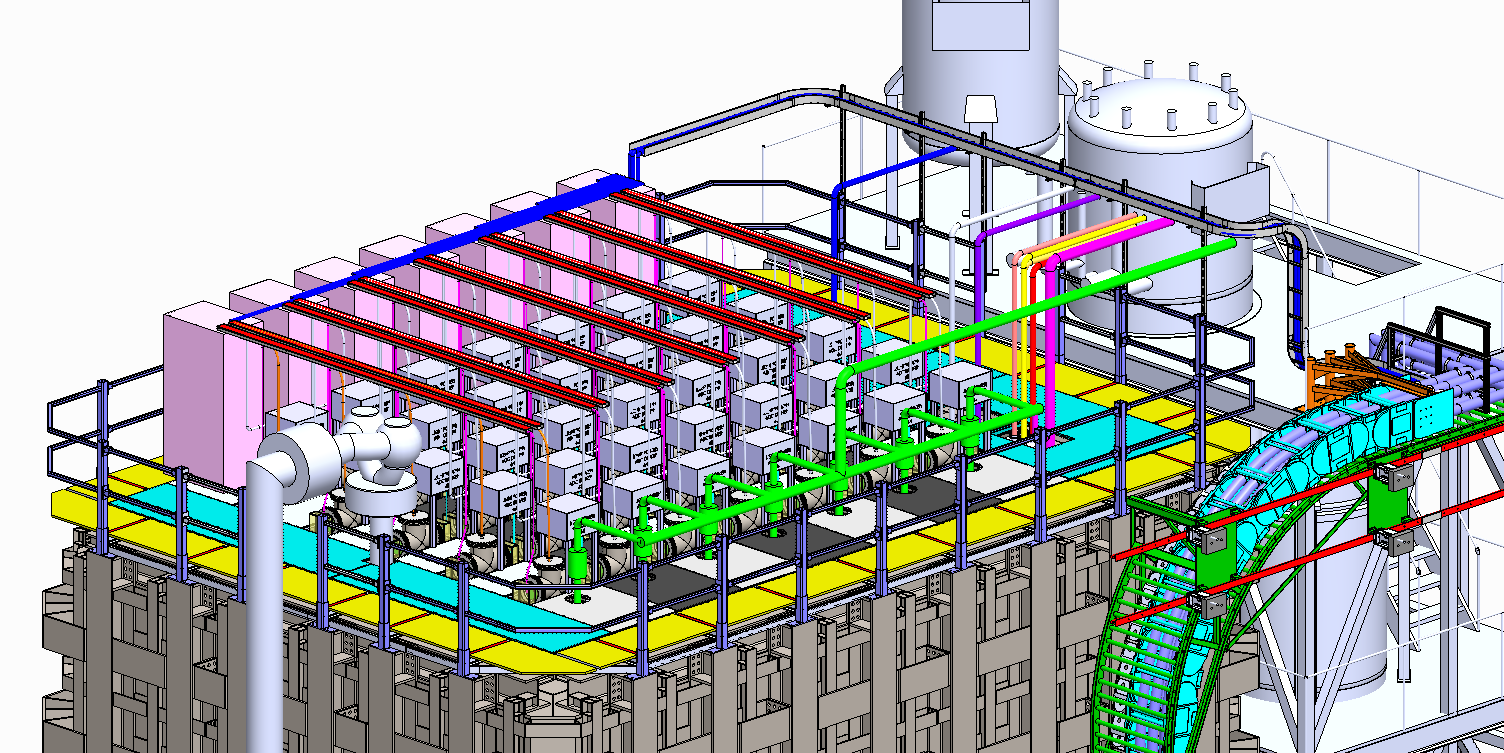
\includegraphics[width=0.95\textwidth]{graphics/cryostat/cryostat-services.png}
%\end{dunefigure}

%%%%%%%%%%%%%%%%%%%%%%%%%%%%%%%%
\section{Risks and Mitigations}
\label{sec:cryost-risks}

Table~\ref{tab:table-cryost-risks} contains a list of all the
risks that \dword{dune} is currently holding in the cryostat risk register.  Each line includes the official \dword{dune} risk register identification number, a description of the risk, the proposed mitigation for the risk, and finally three columns rating the post-mitigation (P)robability that the risk described comes to pass, the degree of (C)ost risk for that line, and the degree of (S)chedule risk.  Risk levels are defined as (L)ow (<10\% probability of occurring, <5\% cost impact, <2 month schedule impact), (M)edium (10 to 25\% probability of occurring, 5\% to 20\% cost impact, 2 to 6 month schedule impact), or (H)igh (>25\% probability of occurring, >20\% cost impact, >6 month schedule impact).  Most of these risks are reduced to a ``Low'' level following mitigation (as shown in the table), although several of them currently hold a higher risk levels (pre-mitigation), due to the early stage of development of the cryostat system relative to other systems.  

In the following sections, we present a narrative description of each of the risks and the proposed mitigation.

\fixme{Anne needs to get risk table template put together}
%\input{generated/risks-longtable-ND-LAr.tex}

\begin{itemize}
\item Membrane cryogen leak
\item Ambient moisture leak
\end{itemize}

\begin{dunetable}
[Placeholder for risks table]
{cc}
{tab:table-cryost-risks}
{Placeholder for Risks Table - it will be generated from a spreadsheet}
Rows & Counts \\ \toprowrule
Row 1 & First \\ \colhline
Row 2 & Second \\ \colhline
Row 3 & Third \\ % no \colhline on final row
\end{dunetable}

%%%%%%%%%%%%%%%%%%%%%%%%%%%%%%%%
\section{Schedule}
\label{sec:cryost-org-sched}

Table \ref{tab:cryost-sched} lists key milestones in the design, validation, construction, and installation of the cryostat.  These milestones include external milestones indicating linkages to the main \dword{dune} schedule (highlighted in color in the table), as well as internal milestones such as design validation and technical reviews.

\fixme{Anne to get list of main DUNE sched items from Eric J before making the real table template}


\begin{itemize}
\item Warm structure
\item Cold structure
\item Composite window
\item Cryostat lid
\item Cryostat integration at Near Site
\end{itemize}

\begin{longtable}
{p{0.75\textwidth}p{0.25\textwidth}}
\caption{Cryostat consortium schedule}\\ \colhline
\rowcolor{dunetablecolor}Milestone & Date   \\ \toprowrule


\rowcolor{dunepeach}Beneficial occupancy of cavern 1 and \dword{cuc}& \cucbenocc      \\ \colhline
Initial batch (80 PD modules) assembled  & March 2023\\ \colhline

\rowcolor{dunepeach}Top of \dword{detmodule} \#1 cryostat accessible& \accesstopfirstcryo      \\ \colhline
Third batch (320 PD modules) arrive at US PD Reception Facility  & January 2024\\ 

\label{tab:cryost-sched}
\end{longtable}

%%%%%%%%%%%%%%%%%%%%%%%%%%%%%%%%
\section{Prototyping Plans}
\label{sec:cryost-proto}

The composite window is a new technology for LAr designs, as previous designs have been constructed of entirely steel framed. This test plan shall validate the composite window as a newer technology by executing multiple test processes.

\subsection{Test Plan Summary}
\label{sec:cryost-proto-test}

The test plan for the composite window will scale in complexity and scale.

Tests will start with validating the materials chosen and the scarf joint which is a critical element
joining the composite window to the steel structure of the cryostat. Due to the size of the window the
materials chosen will need to be validated to ensure the fabrication process will be successful.

After the scarf joint is validated, tests will move onto sandwich beam tests. Tests will be performed
to understand cantilever bending strength in the sandwich. Additionally, there are a significant
amount of non-mechanical tests to be performed with these samples that will assist in integration.
Finally a composite plate that closely reassembles the real window, but on smaller scale will be
fabricated. This will be put under pressure for gas tightness and hydrostatic loading.
As such, these tests are split into 4 main categories. MATERIAL, JOINT, BEAM, and PLATE

\begin{enumerate}
    \item MATERIAL TESTS
    \begin{itemize}
        \item RTM (VARTM) FLOW LENGTH \& TIME VALIDATION
    \end{itemize}
    \item JOINT TESTS
    \begin{itemize}
        \item TENSILE COUPON TEST - Fabricated and Tested in accordance to ASTM D3039
        \item COMPRESSION COUPON TEST - Fabricated and Tested in accordance to ASTM D3410
        \item TENSILE COUPON TEST AT COLD - Fabricated and Tested in accordance to ASTM D3039 near LN2 temperatures
        \item COMPRESSION COUPON TEST AT COLD - Fabricated and Tested in accordance to ASTM D3410 near LN2 temperatures
    \end{itemize}
    \item BEAM TESTS (Full Thickness)
    \begin{itemize}
        \item CANTILEVER BEAM LOADING
        \item WELDING PROXIMITY INTEGRATION TEST
        \item THERMAL CYCLING
        \item OPTIONAL: FLAMABILITY
    \end{itemize}
    \item PLATE TESTS (Scaled Thickness + Size)
    \begin{itemize}
        \item PRESSURE LOAD TEST
    \end{itemize}
\end{enumerate}

\subsection{Material Validation}
\label{sec:cryost-proto-matval}

There are key considerations for material when fabricating a window of this size. Firstly the size itself is very large which means fabricating inside an autoclave in one-piece is near impossible. This
means it needs to be made outside an autoclave and oven, thus a room temperature cure.
Additionally due to the size the RTM method must be validated to allow resin to penetrate the entire
length of the window. As seen in the figure below, if resin does not travel sufficient distance in the
cure time then the part does not become fully wetted. The most common civil engineering works for
composites will be performed by pultrusion or vacuum assisted resin transfer molding (VARTM /
RTM).  A resin travel vs time test is shown in Figure \ref{fig:cryostat-protoresin}.

\begin{dunefigure}[Resin travel vs cure time]{fig:cryostat-protoresin}
{Different RTM test samples showing resin travel over cure time.}
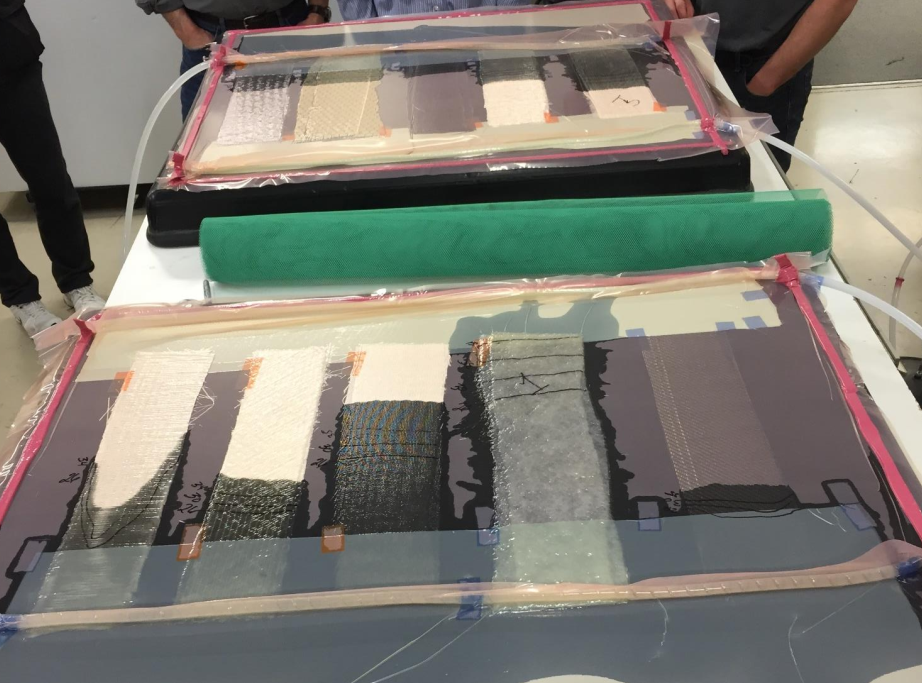
\includegraphics[width=0.95\textwidth]{graphics/cryostat/cryostat-protoresin.PNG}
\end{dunefigure}

Ideal manufacturing processes:

\begin{itemize}
    \item Room Temperature Cure
    \item Not limited by size (Does not need to fit in autoclave or oven)
    \item Slow Cure (to allow resins to fully transfer through fibers)
    \item Can be manufactured without significant equipment (does not require specialized facility)
\end{itemize}

The composite window can be split in a few main subcomponents.

Fiber: The fiber is expected to be glass fiber. However many different specifications exists for a
recommended type of fiberglass. E-glass or R-glass fibers. Additionally this fiber should have very
high fiber aerial weight to increase thickness quickly without excess number of layers. (25mm
thickness with approx. 100 layers at 0.25 per layer).

Resin: Resins should be room temp cure with a long pot life. Tg exceeding 60C.

\begin{itemize}
    \item TotalBoat
    \item Entropy
    \item West Systems
    \item Hexion
\end{itemize}

Epoxy Resins will likely be a more applicable choice. Although Polyester and Vinyl Ester resins are
recommended in many specs, they are unlikely to meet our requirements.

Core: Core should have a density of 90kg/m3 or higher. E= 10MpA. V = 0.5 (incompressible). Balsa
wood is the base material.

\subsection{Scarf Joint Validation}
\label{sec:cryost-proto-scarfval}

\subsubsection{Tensile Properties}
\label{sec:cryost-proto-scarften}

\begin{dunefigure}[Coupon dimensions]{fig:cryostat-coupon}
{Coupon dimensions.}
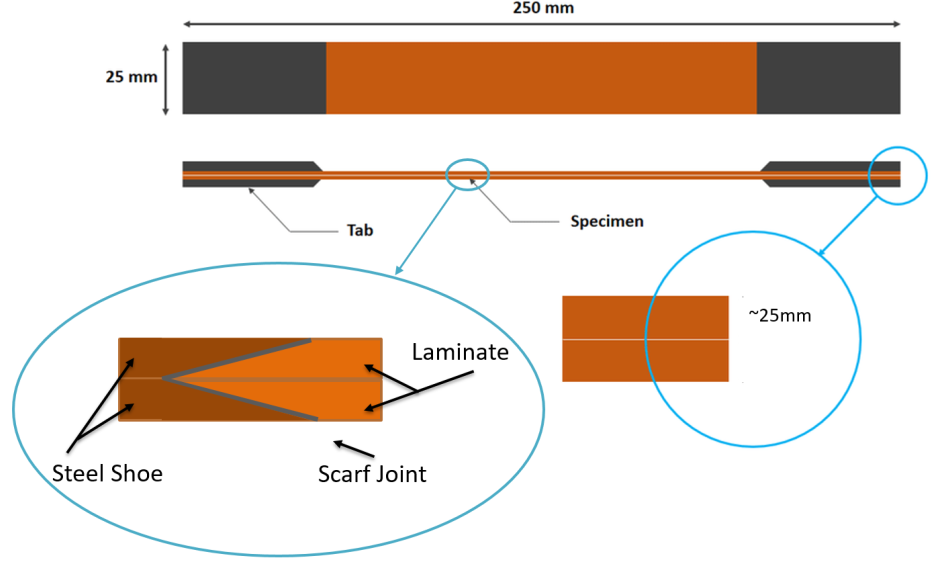
\includegraphics[width=0.95\textwidth]{graphics/cryostat/cryostat-coupon.PNG}
\end{dunefigure}

Coupon dimensions are derived from ASTM standards. The non-standard feature being tested is the
scarf joint within the laminate.

Complete testing guidelines for tensile properties of composite coupons are described by ASTM
D3039 Standard Test Method for Tensile Properties of Polymer Matrix Composite Materials. The test
standard defines length and width requirements for the samples. A common recommended size for
these samples are 250mm by 25mm, with 25mm on each end being a bonded metal tab. The
complete details of this test are not be transcribed into this test plan. However, the general test
process is:

\begin{enumerate}
    \item Create standardized test coupons.
    \item Bond metallic tabs to the coupons. This reduces possible ‘crushing’ of the fibers when put
into a universal test machine.
    \item Apply tensile force using test machine. The machine will measure deflection and load applied.
    \item Save stress/strain curve and load/deflection values.
\end{enumerate}

The fracture load is of specific interest to us. We expect this load to exist within the laminate and not the joint.

\subsubsection{Compression Properties}
\label{sec:cryost-proto-scarfcomp}

Coupon sized for compression testing are slightly different. Width is still 25mm, length ~150mm with
tabs of 65mm.

The complete test standard is contained within ASTM D3410 Standard Test Method for Compressive
Properties of Polymer Matrix Composite Materials with Unsupported Gage Section by Shear
Loading[2]. The complete details of this test are not be transcribed into this test plan. The goal of the test is much the same as the tensile test, which is to develop a stress-strain curve.

\subsubsection{Tensile Properties at Cold Temperature}
\label{sec:cryost-proto-scarftencold}

Tensile properties at cold temperature follow the exact same standards are the Tensile Test.
However, test samples will be subjected to load at near LN2 temperatures. This can be done using
a thermal chamber, LN2 bath while under load, or have the test specimens removed from a LN2
bath then quickly inserted into the test setup.

There are thermal chambers available that can provide hot or cold temperatures to samples while
under load. Ideally the test provider will have a chamber unavailable. Understandably this
equipment requires significant investment. As such, LN2 bath would also be sufficient to provide
cold temperatures.

There are strategies to surround the sample in LN2 bath while under load. However, even simpler
is to soak the test samples prior to the test and simply monitor temperature while load is applied.
This strategy should be agreed upon with safety committees.

\subsubsection{Compression Properties at Cold Temperature}
\label{sec:cryost-proto-compression}

The compression test at cold is exactly the same as the D3410 compression standard, however also includes cold bath strategies described in the previous section.

\subsubsection{Laminate Properties - No Scarf Joint}
\label{sec:cryost-proto-noscarften}

The laminate-only properties will be critical for comparison of strength to test coupons that contain
the scarf joint. The same tests will be performed using a series of laminate-only coupons that do not
contain the scarf joint.

\subsection{Sandwich Beam Properties}
\label{sec:cryost-proto-sandbeam}

\subsubsection{Manufacturing}
\label{sec:cryost-proto-sandbeam-manu}

The Sandwich Beam samples will be manufactured as full thickness, but reduced width and length.

\begin{dunefigure}[Beam construction and dimensions]{fig:cryostat-sandwich}
{Beam construction and dimensions.}
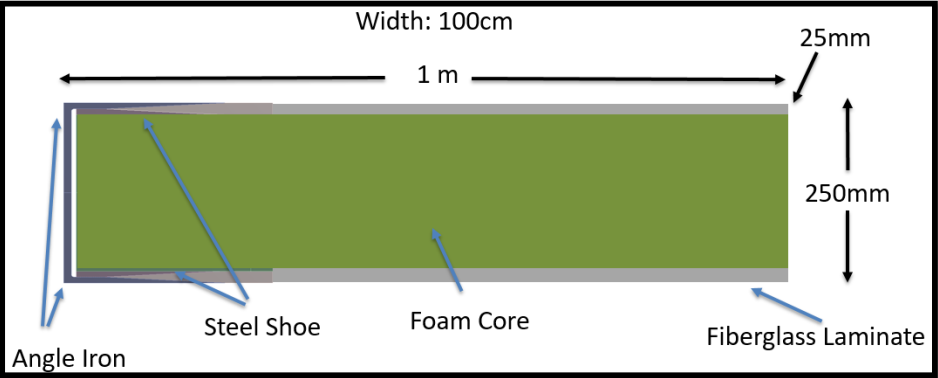
\includegraphics[width=0.95\textwidth]{graphics/cryostat/cryostat-sandwich.PNG}
\end{dunefigure}

There are many unanswered process questions regarding the construction of a sandwich plate
with steel joints. Many of these questions will be answered at this time of prototype manufacturing.
A detailed construction process will be followed and recorded such that a lessons learned can be
applied to fabrication of the full-scale window.

\subsubsection{Beam Loading}
\label{sec:cryost-proto-sandbeam-load}

Beam Loading will be applied as cantilever and measured with strain gauges are multiple locations
along the length of the beam. The load applied is a representative point load based on the hydrostatic
load the entire plate will experience (estimated 3bar hydrostatic load). This loading will be compared
to a sub-model analysis which will further validate the analytical model.

\begin{dunefigure}[Beam loading configuration]{fig:cryostat-sandwich-2}
{Beam loading configuration.}
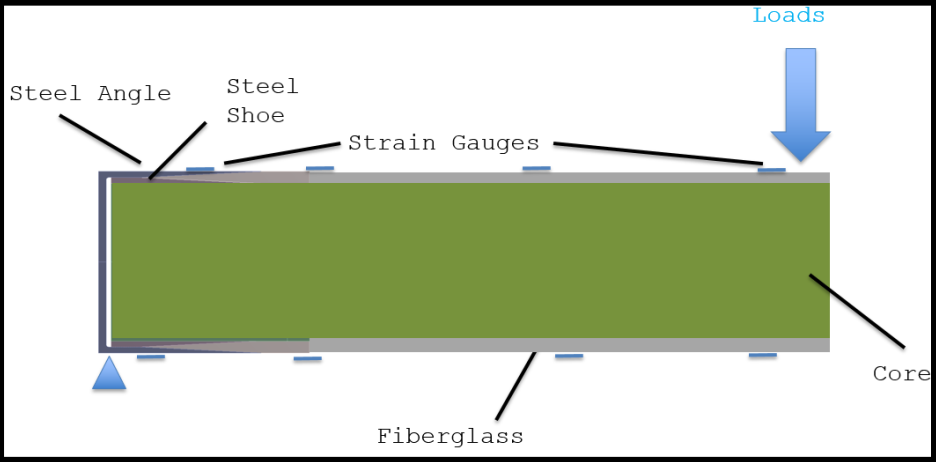
\includegraphics[width=0.95\textwidth]{graphics/cryostat/cryostat-sandwich-2.PNG}
\end{dunefigure}

Load will also be applied as representative deflection at a value 1m from the edge of the plate within
the analytical model. This measurement will also further validate the analytical model.

\subsubsection{Welding Validation}
\label{sec:cryost-proto-sandbeam-weldval}

In addition to material construction, there are concerns regarding integration between steel
structures and composite materials. A majority of the detector is made from steel beams which will
be connected to the steel framed composite window. This will likely be performed in some part with
welding. Fiberglass, foam, and adhesives may not perform well near proximity of welding. A series
of studies shall be performed to study a safe distance to weld from the fiberglass, foam core, and
adhesive scarf joint locations.

To address a concern of composite sandwich integrity when exposed to the cold temperatures of
liquid argon within the cryostat a series of tests may be performed on a sandwich beam. This can be
tested with two samples. The first control sample which is not subjected to any cold temperature.
Then a second sample which would be submerged into LN2 temperatures prior to testing.
The tests to qualify integrity are based on a subset of ASTM C481 Standard Test Method for
Laboratory Aging of Sandwich Constructions (need Ref).

\begin{itemize}
    \item Shear Test: Test Method C273
    \item Compressive Strength: Test Method C364 and C365/C365M
    \item Delamination Strength: Test Method C363
    \item Tensile Strength: Test Method C297/C297M
    \item Flatwise Flexure: Test Method C393
    \item Climbing Drum Peel Test Method D1781
\end{itemize}

\subsection{Window Plate Properties}
\label{sec:cryost-proto-winplate-prop}

The final test to validate the composite window readiness level will be a subscale composite window.
The size of the window is meant to be as large as possible without making manufacturing or testing
significantly challenging. The scale chosen for this is 1/4
The window will undergo hydrostatic loading using pressurized air. Currently this is calculated using
350mBar of H20 and 4.5 meter tall Argon for a 1 bar load. With a safety of factor of 3, this is 3 bar or
43.5 psi. To perform this testing, a sealed steel box will be made that interfaces to the composite
window and simulates the remaining structure of the cryostat. It will then be pressurized to 3bar.
Stress/Strain on the window will be measured using strain gauges.
Additionally this test allows a measurement of leak rate. The composite window is ideally gas tight.
That will be verified here by installing pressure gauges to the simulated structure.
This simulated build also allows development of Nondestructive Testing methods to ensure quality
on the full-scale window build.

%%%%%%%%%%%%%%%%%%%%%%%%%%%%%%%%
\section{Construction Plans}
\label{sec:cryost-construc}

\subsection{PRISM Frame Installation}
\label{sec:cryost-construc-PRISMFrame}

The PRISM frame consists of three major subassemblies which will be delivered to the surface of the site and lowered into the cavern before being bolted together. After mounting the frame to the PRISM rollers, a layer of self leveling epoxy will be used on the top of the frame to provide a level support for the warm structure.

\subsection{Warm Structure Installation}
\label{sec:cryost-construc-warm}

The warm structure subassemblies will be delivered to the surface of the site and lowered into the cavern for final assembly. Design of the subassemblies is still in progress but will consist generally of partial width wall sections, partial width bottom sections and edge sections. First the bottom sections will be placed on top of the PRISM frame, followed by edge and wall sections. Installation will consist of structural bolted joints and gas tight welding of the inner skin of each wall section.

The composite window is best suited to surface assembly and will therefore be assembled into its corresponding steel support structure on the surface before being lowered into the cavern. First, a fiberglass face sheet will be bonded to a frame of steel beams. Then, the polyurethane foam core will be bonded to the face sheet. Next, a second face sheet and set of steel beams will be bonded to the free side of the core. Finally, the beams of the steel window frame will be welded together to complete the window assembly. The window will then be lowered into the cavern for integration into the rest of the warm structure.

\subsection{Cold Structure Installation}
\label{sec:cryost-construc-cold}

Installation of the cold structure will be completed by the membrane supplier and will follow their standard operating procedure.  Broadly, it will consist of the following steps:

\begin {itemize}
\item Welding of stainless steel support rods on the vapor barrier of the warm structure to support the insulation and membrane during installation.
\item Application of mastic adhesive which will provide a bond between the first layer of insulation and the vapor barrier.
\item Installation of layers of insulation, secondary containment barrier and supporting hardware until the desired thickness is achieved.
\item Installation of corrugated membrane sections, held by support rods and welded to each other.
\end{itemize}

\subsection{\dword{ndlar} Cryostat Lid Installation}
\label{sec:cryost-construc-cold-lid}

The first lid section installed provides cryogenic services to the \dword{ndlar} cryostat.  The cryo-services section is lowered into the cryostat and positioned at the end closest to the cryogenics mezzanine.  Temporary support structures are installed to support the lid for the installation process, as well as temporary work platforms.  Once the cryo-services section is firmly secured, a weld seam is placed around the perimeter of the lid, sealing it with the cryostat main body vapor seal; seal integrity is verified via localized helium leak check.  Once the seal is complete and verified, structural brackets are installed to mechanically anchor the cryo-services section to the cryostat main body, see Figure \ref{fig:cryostat-cryoservweld}.  Cryogenic services are then routed inside the cryostat; these are leak checked prior to subsequent \dword{lartpc} row installation.

\begin{dunefigure}[\dword{ndlar} cryostat cryogenics services]{fig:cryostat-cryoservweld}
{Cryogenc section weld seal.}
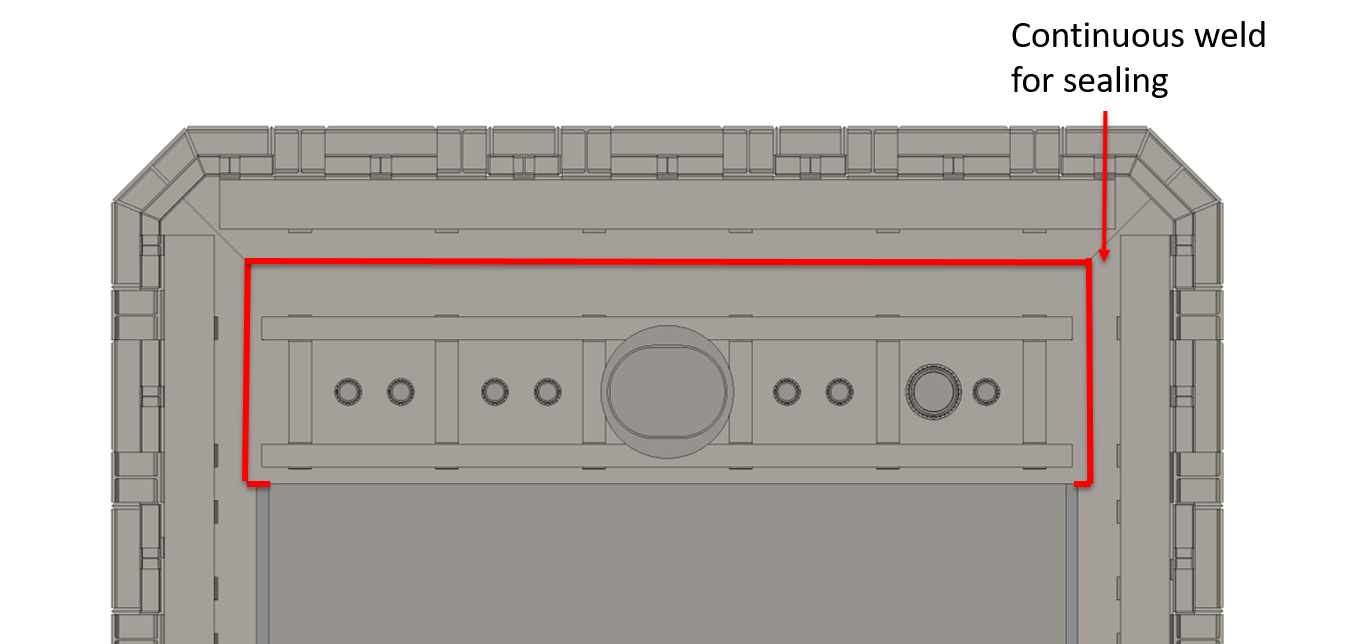
\includegraphics[width=0.65\textwidth]{graphics/cryostat/cryostat-cryoservweld.png}
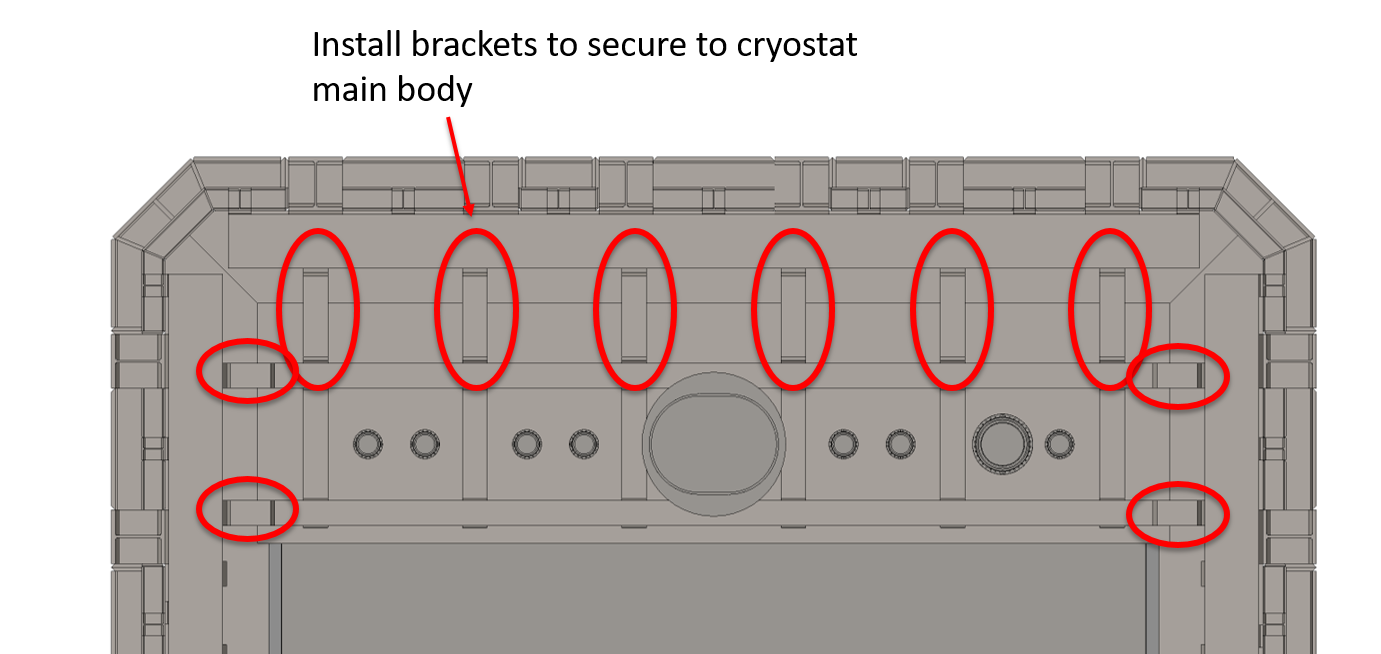
\includegraphics[width=0.65\textwidth]{graphics/cryostat/cryostat-cryoservbrack.png}
\end{dunefigure}

%\begin{dunefigure}[LArTPC section cryostat lid]{fig:cryostat-cryoservebrack}
%{Cryogenic section bracket installation.}
%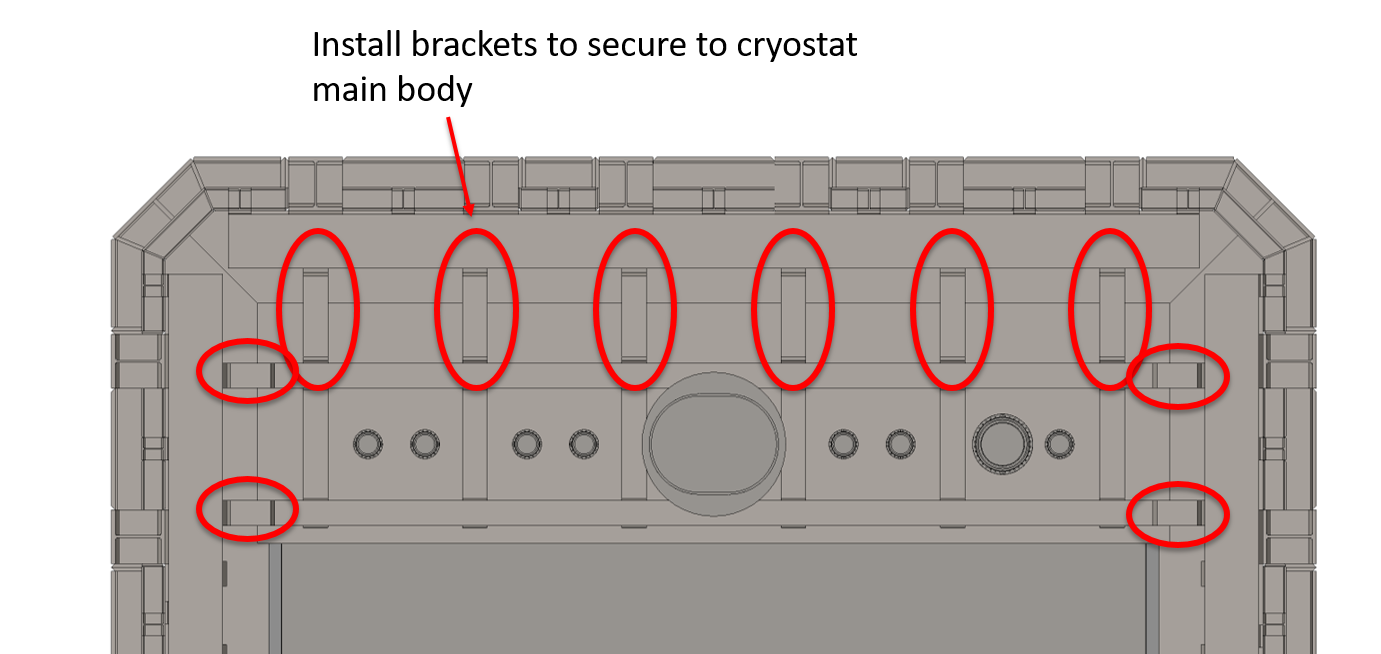
\includegraphics[width=0.75\textwidth]{graphics/cryostat/cryostat-cryoservbrack.png}
%\end{dunefigure}

After the cryogenic section installed has finished, the \dword{lartpc} detector sections are sequentially installed to the main body of the cryostat.  Similar to the cryo-services section, each \dword{lartpc} lid section is lowered into position, as seen in \ref{fig:cryostat-modrowinstall}. 

\begin{dunefigure}[\dword{lartpc} section cryostat lid]{fig:cryostat-modrowinstall}
{\dword{lartpc} row installation.}
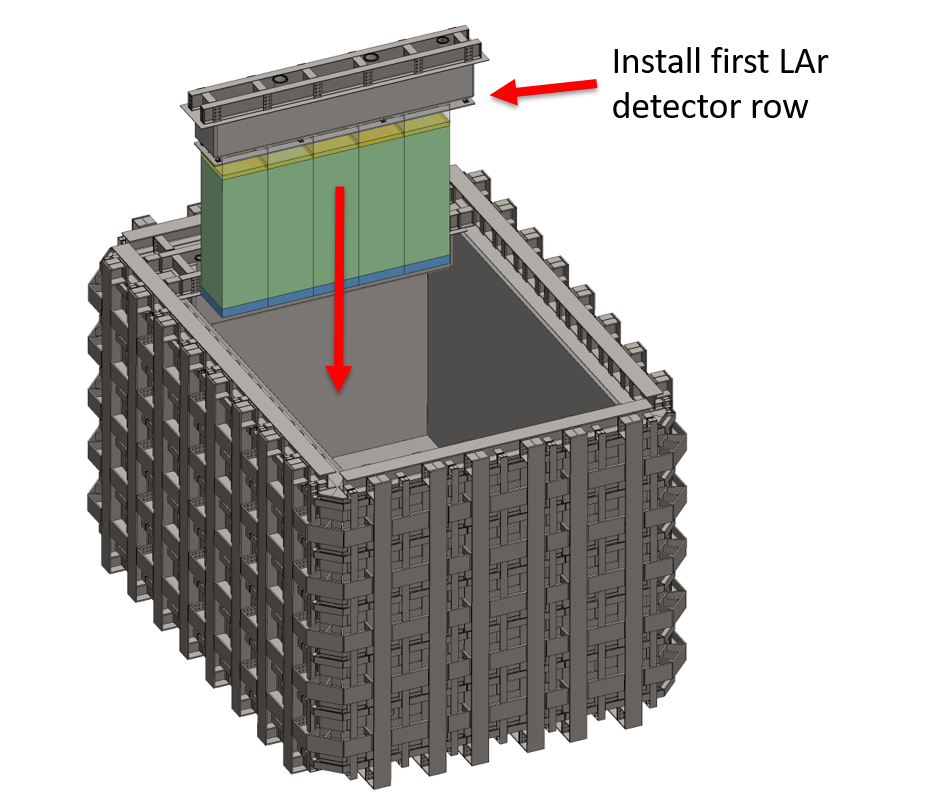
\includegraphics[width=0.65\textwidth]{graphics/cryostat/cryostat-modrowinstall.png}
\end{dunefigure}

After the first row installation special oversight is required for subsequent row installation due to the small clearance envelopes between adjacent rows.  Once each section is lowered in, temporary support structures are installed along with required work platforms. At this point final warm acceptance checks are done for each module row.  After final checks complete, a weld seam is again laid down around the perimeter of the lid section to seal to the cryostat main body and adjacent lid section; seal integrity is helium leak checked.  After seal integrity is verified the structural brackets are installed to secure the lid section to the cryostat walls and any adjacent lid sections as shown in Figure \ref{fig:cryostat-modweld}.

\begin{dunefigure}[Cryostat cryogenics services]{fig:cryostat-modweld}
{LArTPC section weld seal.}
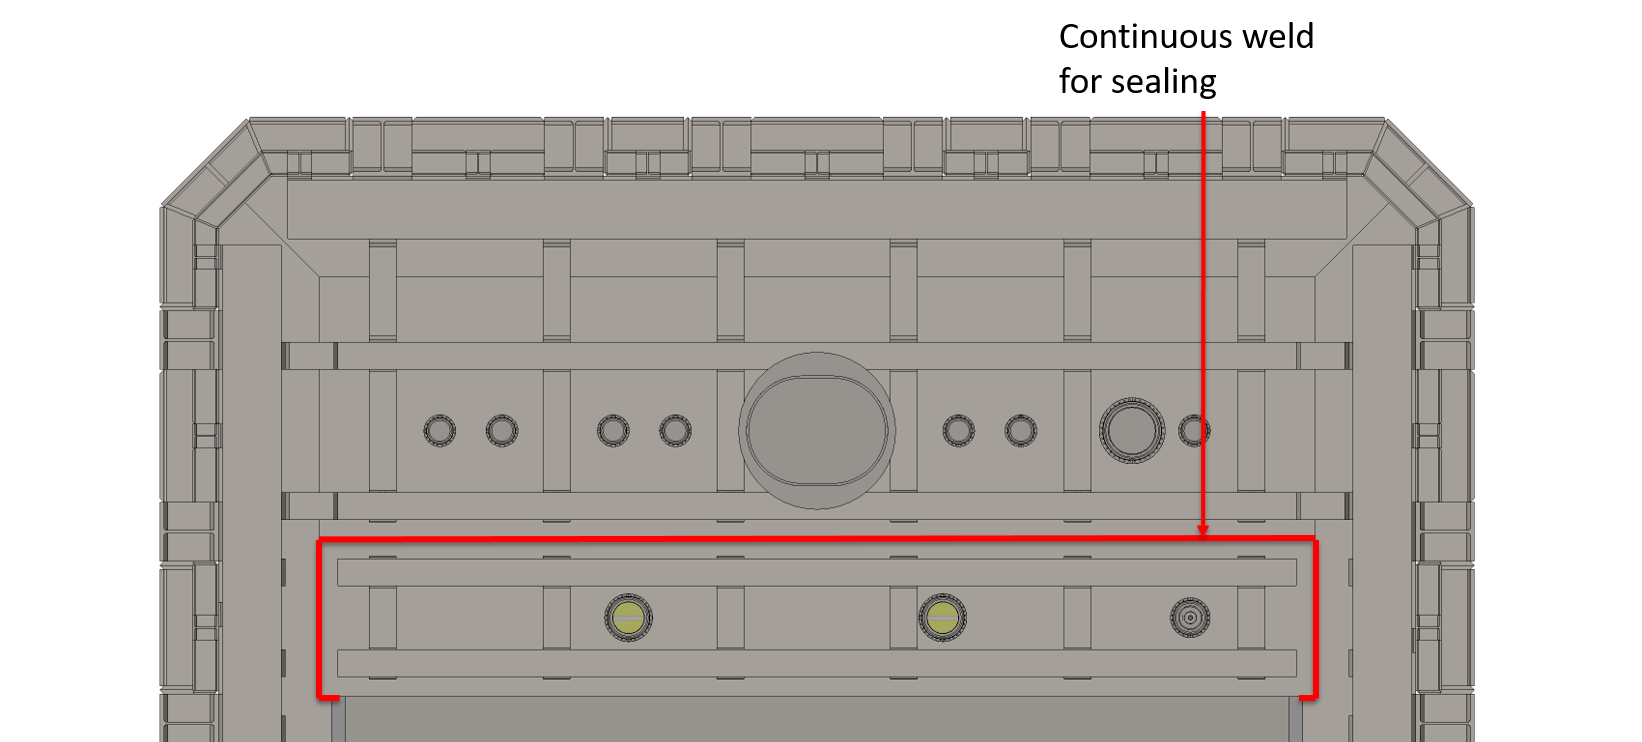
\includegraphics[width=0.65\textwidth]{graphics/cryostat/cryostat-modweld.png}
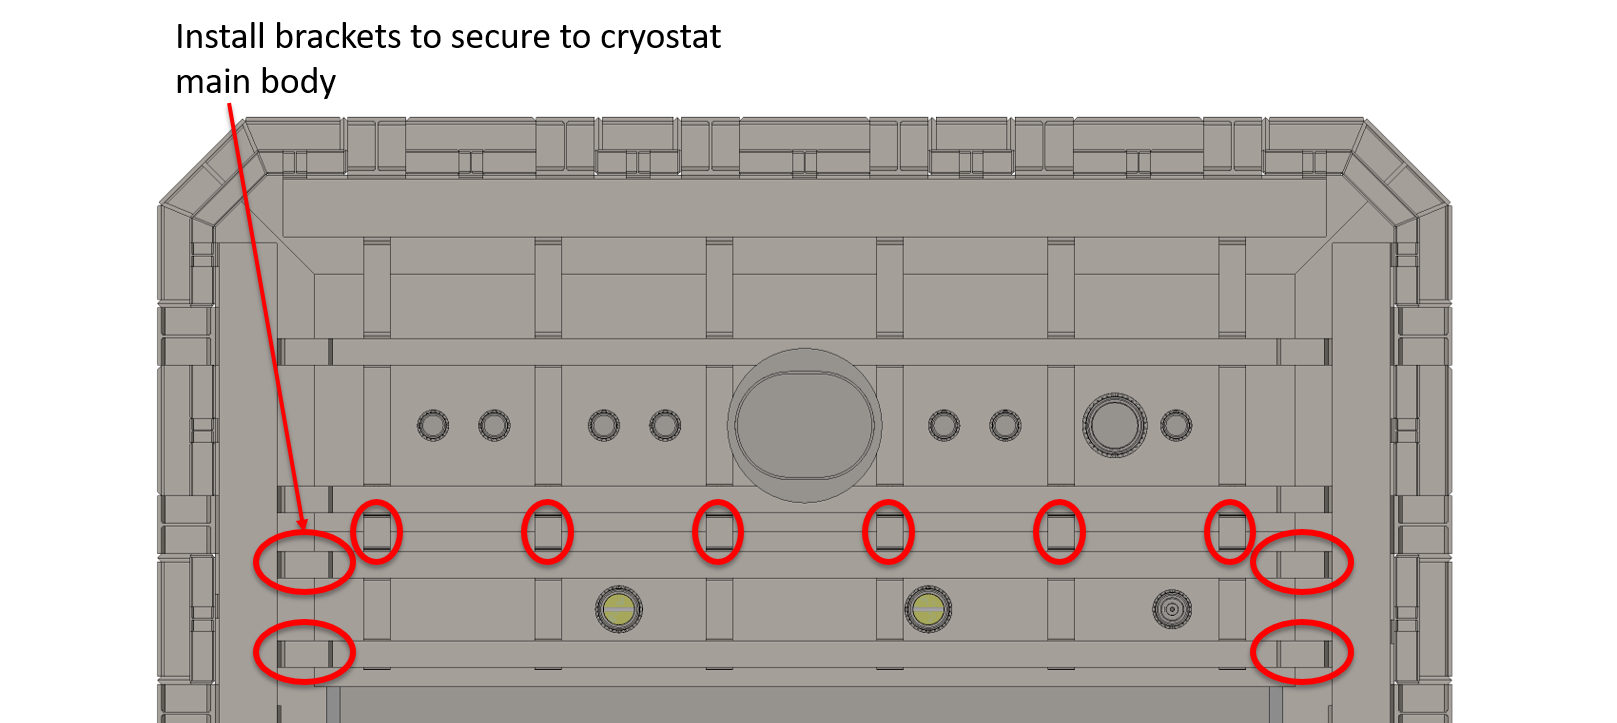
\includegraphics[width=0.65\textwidth]{graphics/cryostat/cryostat-modbrack.png}
\end{dunefigure}

%\begin{dunefigure}[LArTPC section cryostat lid]{fig:cryostat-modbrack}
%{LArTPC section bracket installation.}
%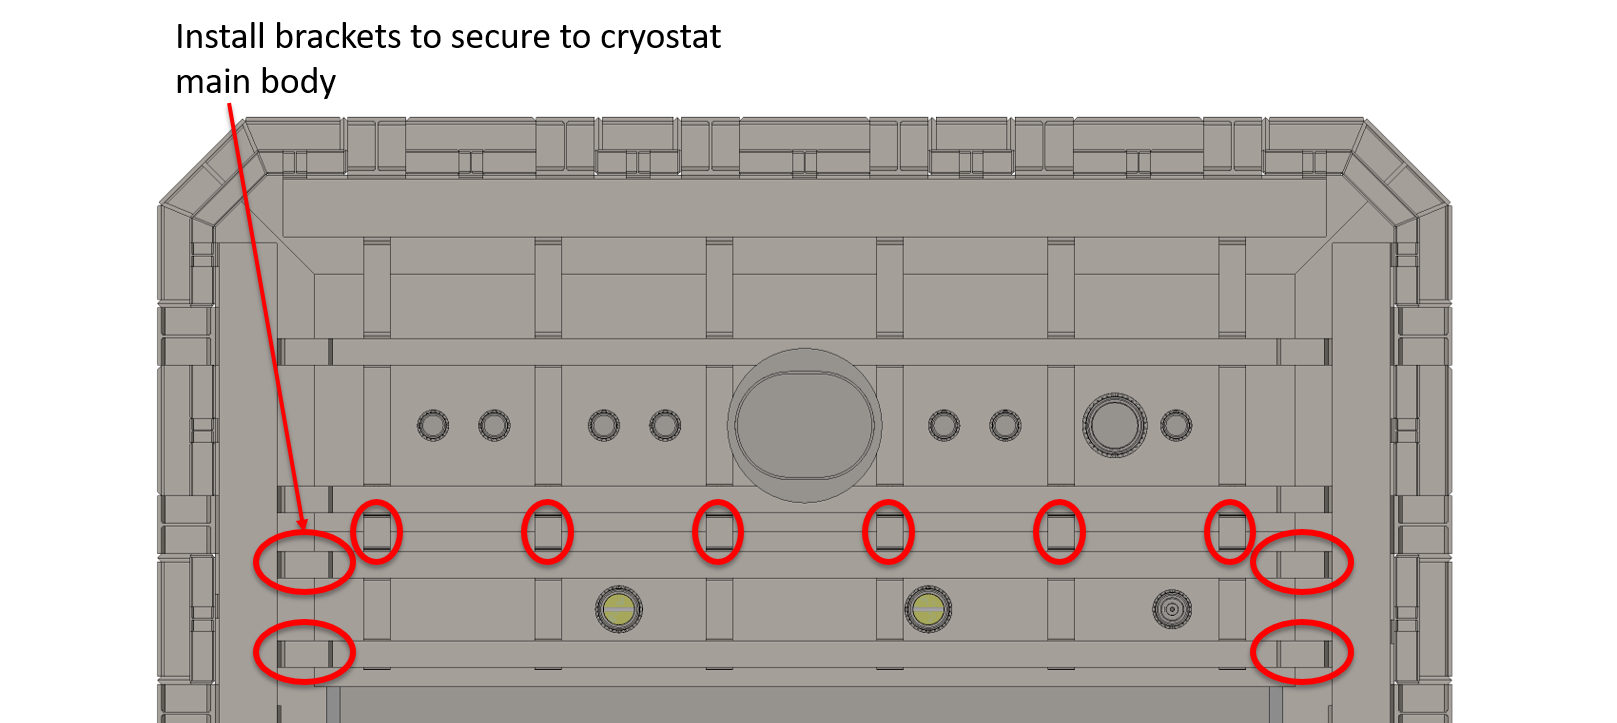
\includegraphics[width=0.75\textwidth]{graphics/cryostat/cryostat-modbrack.png}
%\end{dunefigure}

The final lid section installed contains the cryostat pressure relief valve.  This section is also intended to be field machined to final dimensions to ensure proper fit.  Similar to the other sections, it is lowered into place and temporary support structures are installed.  A weld seam is laid down around the perimeter to create the final seal of the cryostat; this seal is again helium leak checked. Brackets are installed to complete load transfer of the full lid section and all temporary support structures are removed.



\subsection{Commissioning}
\label{sec:cryost-construc-commiss}

The tests described below are performed to qualify the warm structure of the cryostat. To proceed from one test stage to the next, the respective authorities of the host laboratory performs an internal review. Their approval is mandatory prior to each test. Prior to each testing campaign:

\begin{itemize}
\item A risk assessment is performed to verify personnel and equipment safety during the tests
\item The safety file related to the phase is complete and validated by the safety authorities
\end{itemize}

The structural static qualification tests are monitored with strain gauges and displacement sensors located on the warm structure of the cryostat. During the tests, the strain gauges and displacement sensors data are compared in real time with the results of the FEA calculations. Any significant deviations from linearity or abnormal stress readings will block the process.

The expected qualification tests are the following: 

\begin{enumerate}
    \item Destructive tests for the weakest structural part of the steel frame are performed to validate the FEA models and the structure mechanical behavior. The weakest connection is identified on the basis of Eurocode 1993 provisions [3]. If required, the FEA models are modified accordingly and an update of the calculations is performed. 
    \item The stiffness and strength tests of the joint between the composite window and the steel structure are described in detail in [10] and will not be treated here.
    \item Structural tests of the window laminate are performed as required by ASME RTP1 [5].
    \item Prior to the Liquid Argon filling process and the start of the cryogenics commissioning phase, a pneumatic test is performed at a testing pressure of 200 mbarg, using warm argon gas. Note that the automatic pressure vent valve is set at 150 mbarg in normal control conditions. This test will: 
    \begin{itemize}
    \item Verify the quality of the cryogenics controls system and procedures, showing the quality and precision of the pressure regulation. 
    \item Validate the FEA analysis and models for 200 mbarg overpressure pure gas load case. If needed, the FEA models will be updated.
    \item Qualify the cryostat structure for 200 mbarg gas overpressure. 
    \end{itemize}

Prior to this pressure test, all feed-through and other external components shall be pressure rated for a design pressure of a least 350 mbarg. The pressure rating shall be obtained through documented qualification process, including design calculations and testing program. Additionally, each feed-through shall be pressure tested prior to installation into the cryostat in an appropriate setup that is described in a separate document. 

    \item Then, the cryostat will be filled with liquid argon in incremental steps until its service level. The cryostat is instrumented with strain gauges and displacement sensors (dial gauges) to monitor strains and stresses and deformations. The structural behavior of the warm structure is checked all along the filling process by continuous reading of the strain gauges and displacement sensors results (at daily basis). In case of abnormal behavior of the structure, (i.e. large variations from simulated data or large asymmetry in the structural behavior), the filling process is stopped. If required, the cryogen is drained.

The gas overpressure to be additionally applied at the top of the liquid level is defined from the cryogenics system requirements and should be lower or similar to agreed operation pressure. 

During the filling of the cryostat, several tests are performed to control the warm structure behavior. Every 2.0 m of LAr level increase in the cryostat, the gas pressure will be increased in steps of 50 mbar up to 200 mbarg. At the beginning of the process (below 4.0 m) measured displacements and deformations may differ (reasonably) from the FEA results. This difference can be related to the initial settling of the structure, likely to occur during the introduction of the first few meters of LAr.

    \item Once the filling has reached the service level, the design gas over-pressure Pt (350 mbarg) will be applied at the top of the liquid level. 
    
The final value of the test over-pressure should be confirmed via the risk assessment of the cryostat and mitigating safety measures. It should remain sufficiently lower than the set up value of the safety valve, in order to avoid any opening or leak of the safety valve. 

    \begin{itemize}
        \item Qualify the cryostat structure for the characteristic load case: cryostat structure full of LAr (service level) + Pt (350 mbarg) argon gas design overpressure. 
        \item Finish the validation of the FEA models and analysis for the operational type of load case (LAr at service level + Pt (350 mbarg) overpressure). In case of need, the FEA models will be updated. 
    \end{itemize}

    \item The measurements performed via step number 5 will be used to qualify the FE models. The data will be used to update the models and run them again. An updated estimate of the maximum loads and stresses will be obtained for the design case (LAr full + 350 mbarg) and a final verification of the European and US regulations ([2], [3]) will be performed.

\end{enumerate}

Any modification of the static FE model will be implemented also on the dynamic model used for dynamic analysis, updating the seismic calculations.

\subsection{References}
\label{sec:cryost-construc-ref}

\begin{enumerate}
\item FESHM 5031.7: Membrane Cryostats
\item ANSI/AISC 360-16 (July 2016): Specification for Structural Steel Buildings
\item Eurocode 1993 (May 2005): Design of steel structures
\item Acceptance of Steel and Aluminum Structures Designed per the Eurocodes at Fermilab
\item ASME RTP-1-2013 - Reinforced Thermoset Plastic Corrosion-Resistant Equipment
\item Eurocode 1990 (April 2002): Basis of structural design
\item Eurocode 1998 (December 2004): Design of structures for earthquake resistance
\item EN-14620 (December 2006): Design and manufacture of site built, vertical, cylindrical, flat-bottomed steel tanks for the storage of refrigerated, liquified gases with operating temperatures between 0 °C and -165° C
\item EN 1090-2: Technical requirements for the execution of steel structures
\item DUNE Doc. DU-1000-XXX – Experimental plan for the qualification of the joints
\end{enumerate}


%\begin{itemize}
%\item Warm structure installation
%  \begin{itemize}
%  \item Steel section assembly
%  \item  Composite wall installation
%  \end{itemize}
%\item Cold structure installation
%  \begin{itemize}
%  \item Primary membrane \& insulation
%  \item  Secondary membrane \& insulation
%  \end{itemize}
%\item Cryostat lid installation
%\item Leak checking
%\item Commissioning
%\end{itemize}

\begin{comment} %% commenting all to the end
\fixme{The following sections are not in the new structure; I'm keeping them at the end here for now, in case you want to include one or more of them later.}
%%%%%%%%%%%%%%%%%%%%%%%%%%%%%%%%Not in Tim's new organization
\section{Safety Concerns}
\label{sec:cryost-safety}

%%%%%%%%%%%%%%%%%%%%%%%%%%%%%%%%Not in Tim's new organization
\section{Calibration}
\label{sec:cryost-calib}

%%%%%%%%%%%%%%%%%%%%%%%%%%%%%%%%Not in Tim's new organization
\section{Quality Assurance}
\label{sec:cryost-qa}

%%%%%%%%%%%%%%%%%%%%%%%%%%%%%%%%Not in Tim's new organization
\section{Transport and Handling}
\label{sec:cryost-transport}

%%%%%%%%%%%%%%%%%%%%%%%%%%%%%%%%Not in Tim's new organization
\section{Installation, Integration, and Commissioning}
\label{sec:cryost-iic}

%%%%%%%%%%%%%%%%%%%%%%%%%%%%%%%%Not in Tim's new organization
\section{Organization}
\label{sec:cryost-org}

%%%%%%%%%%%%%%%Not in Tim's new organization
\subsection{Participating Institutions}
\label{sec:fdsp-org-inst}
%\metainfo{\color{red}\bf  Content: Segreto/Warner}

The cryostat consortium benefits from the contributions of many institutions and facilities in \fixme{several countries? or the U.S. and ??}.  Table~\ref{tab:cryost-institutes}
lists the member institutions. 

\begin{longtable}
{ll}
\caption{Cryostat consortium institutions}\\ \colhline
\rowcolor{dunetablecolor} Member Institute  &  Country       \\  \toprowrule
univ 1 &  \\ \colhline
univ 2 &  \\ \colhline
univ 3 &  \\ 
\label{tab:cryost-institutes}
\end{longtable}

\end{comment}










